% main.tex — Master document
% AI Workflow Solutions towards the Efficient Preservation of
% Immersive and Intangible Cultural Heritage in Virtual Spaces
%
% Dr John O'Hare, DreamLab AI Consulting Ltd
% For: Roger McKinley, University of Salford
% March 2026

\documentclass[a4paper,11pt,twoside,openright]{report}

% ────────────────────────────────────────────────────────────
% Language and encoding
% ────────────────────────────────────────────────────────────
\usepackage[utf8]{inputenc}
\usepackage[T1]{fontenc}
\usepackage[british]{babel}
\usepackage{microtype}

% ────────────────────────────────────────────────────────────
% Page geometry
% ────────────────────────────────────────────────────────────
\usepackage[
  a4paper,
  top=30mm,
  bottom=30mm,
  inner=30mm,
  outer=25mm,
  headheight=14pt
]{geometry}

% ────────────────────────────────────────────────────────────
% Fonts
% ────────────────────────────────────────────────────────────
\usepackage{lmodern}
\usepackage{inconsolata}

% ────────────────────────────────────────────────────────────
% Colours
% ────────────────────────────────────────────────────────────
\usepackage[dvipsnames,svgnames,x11names]{xcolor}

\definecolor{UoSRed}{HTML}{B71234}
\definecolor{DreamLabAccent}{HTML}{6366F1}
\definecolor{DarkBg}{HTML}{0F172A}
\definecolor{MidGrey}{HTML}{64748B}
\definecolor{LightGrey}{HTML}{F1F5F9}
\definecolor{CodeBg}{HTML}{1E293B}
\definecolor{SuccessGreen}{HTML}{22C55E}
\definecolor{WarningAmber}{HTML}{F59E0B}

% ────────────────────────────────────────────────────────────
% Graphics and figures
% ────────────────────────────────────────────────────────────
\usepackage{graphicx}
\graphicspath{{figures/}{diagrams/}}
\usepackage{subcaption}
\usepackage{float}
\usepackage{wrapfig}

% ────────────────────────────────────────────────────────────
% TikZ and pgfplots
% ────────────────────────────────────────────────────────────
\usepackage{tikz}
\usetikzlibrary{
  calc,
  positioning,
  arrows.meta,
  shapes.geometric,
  decorations.markings,
  backgrounds,
  fit,
  patterns,
  shadows,
  fadings
}
\usepackage{pgfplots}
\pgfplotsset{compat=1.18}

% ────────────────────────────────────────────────────────────
% Tables
% ────────────────────────────────────────────────────────────
\usepackage{booktabs}
\usepackage{tabularx}
\usepackage{longtable}
\usepackage{multirow}
\usepackage{array}
\newcolumntype{L}[1]{>{\raggedright\arraybackslash}p{#1}}
\newcolumntype{C}[1]{>{\centering\arraybackslash}p{#1}}
\newcolumntype{R}[1]{>{\raggedleft\arraybackslash}p{#1}}

% ────────────────────────────────────────────────────────────
% Bibliography
% ────────────────────────────────────────────────────────────
\usepackage[
  backend=biber,
  style=authoryear-comp,
  sorting=nyt,
  maxbibnames=99,
  maxcitenames=2,
  giveninits=true,
  uniquename=init,
  url=true,
  doi=true,
  isbn=false,
  eprint=false
]{biblatex}
\addbibresource{references.bib}

% ────────────────────────────────────────────────────────────
% Hyperlinks
% ────────────────────────────────────────────────────────────
\usepackage[
  colorlinks=true,
  linkcolor=UoSRed,
  citecolor=DreamLabAccent,
  urlcolor=DreamLabAccent,
  bookmarks=true,
  bookmarksnumbered=true,
  pdfauthor={Dr John O'Hare},
  pdftitle={AI Workflow Solutions for Cultural Heritage Preservation},
  pdfsubject={3D Gaussian Splatting for Intangible Cultural Heritage},
  pdfkeywords={Gaussian Splatting, Cultural Heritage, Digital Preservation, AI}
]{hyperref}
\usepackage{bookmark}

% ────────────────────────────────────────────────────────────
% Headers and footers
% ────────────────────────────────────────────────────────────
\usepackage{fancyhdr}

\pagestyle{fancy}
\fancyhf{}
\fancyhead[LE]{\small\textcolor{MidGrey}{\leftmark}}
\fancyhead[RO]{\small\textcolor{MidGrey}{\rightmark}}
\fancyfoot[LE,RO]{\small\textcolor{MidGrey}{\thepage}}
\fancyfoot[CE,CO]{\small\textcolor{MidGrey}{DreamLab AI Consulting Ltd}}
\renewcommand{\headrulewidth}{0.4pt}
\renewcommand{\footrulewidth}{0.2pt}
\renewcommand{\headrule}{\hbox to\headwidth{\color{UoSRed}\leaders\hrule height \headrulewidth\hfill}}
\renewcommand{\footrule}{\hbox to\headwidth{\color{LightGrey}\leaders\hrule height \footrulewidth\hfill}}

\fancypagestyle{plain}{%
  \fancyhf{}
  \fancyfoot[LE,RO]{\small\textcolor{MidGrey}{\thepage}}
  \renewcommand{\headrulewidth}{0pt}
  \renewcommand{\footrulewidth}{0.2pt}
}

% ────────────────────────────────────────────────────────────
% Code listings
% ────────────────────────────────────────────────────────────
\usepackage{listings}
\lstset{
  basicstyle=\ttfamily\small,
  backgroundcolor=\color{LightGrey},
  frame=single,
  rulecolor=\color{MidGrey},
  breaklines=true,
  breakatwhitespace=true,
  showstringspaces=false,
  tabsize=2,
  captionpos=b,
  numbers=left,
  numberstyle=\tiny\color{MidGrey},
  keywordstyle=\color{DreamLabAccent}\bfseries,
  commentstyle=\color{MidGrey}\itshape,
  stringstyle=\color{SuccessGreen}
}

% ────────────────────────────────────────────────────────────
% Coloured boxes (tcolorbox)
% ────────────────────────────────────────────────────────────
\usepackage[most]{tcolorbox}

% Key Finding box
\newtcolorbox{keyfinding}[1][]{%
  enhanced,
  colback=UoSRed!5,
  colframe=UoSRed,
  fonttitle=\bfseries,
  title={Key Finding},
  left=6mm,
  sharp corners=south,
  boxrule=0.8pt,
  toptitle=2mm,
  bottomtitle=2mm,
  attach boxed title to top left={xshift=10mm, yshift=-\tcboxedtitleheight/2},
  boxed title style={
    colback=UoSRed,
    colframe=UoSRed,
    sharp corners,
    size=small
  },
  #1
}

% Recommendation box
\newtcolorbox{recommendation}[1][]{%
  enhanced,
  colback=DreamLabAccent!5,
  colframe=DreamLabAccent,
  fonttitle=\bfseries,
  title={Recommendation},
  left=6mm,
  sharp corners=south,
  boxrule=0.8pt,
  toptitle=2mm,
  bottomtitle=2mm,
  attach boxed title to top left={xshift=10mm, yshift=-\tcboxedtitleheight/2},
  boxed title style={
    colback=DreamLabAccent,
    colframe=DreamLabAccent,
    sharp corners,
    size=small
  },
  #1
}

% Technical Note box
\newtcolorbox{technote}[1][]{%
  enhanced,
  colback=CodeBg!5,
  colframe=MidGrey,
  fonttitle=\bfseries\color{white},
  title={Technical Note},
  left=6mm,
  boxrule=0.6pt,
  toptitle=2mm,
  bottomtitle=2mm,
  attach boxed title to top left={xshift=10mm, yshift=-\tcboxedtitleheight/2},
  boxed title style={
    colback=MidGrey,
    colframe=MidGrey,
    sharp corners,
    size=small
  },
  #1
}

% ────────────────────────────────────────────────────────────
% Glossaries and index
% ────────────────────────────────────────────────────────────
\usepackage[acronym,toc,nonumberlist]{glossaries}
\makeglossaries

\newacronym{3dgs}{3DGS}{3D Gaussian Splatting}
\newacronym{sfm}{SfM}{Structure from Motion}
\newacronym{tsdf}{TSDF}{Truncated Signed Distance Function}
\newacronym{ich}{ICH}{Intangible Cultural Heritage}
\newacronym{uos}{UoS}{University of Salford}
\newacronym{sam}{SAM}{Segment Anything Model}
\newacronym{nerf}{NeRF}{Neural Radiance Fields}
\newacronym{mrnf}{MRNF}{Mini-Splatting with Relocation and Normal Filtering}
\newacronym{mcmc}{MCMC}{Markov Chain Monte Carlo}
\newacronym{usd}{USD}{Universal Scene Description}
\newacronym{webgl}{WebGL}{Web Graphics Library}
\newacronym{colmap}{COLMAP}{COLlaborative MAPping}
\newacronym{ke}{KE}{Knowledge Exchange}
\newacronym{cop}{CoP}{Community of Practice}
\newacronym{gpu}{GPU}{Graphics Processing Unit}

\usepackage{makeidx}
\makeindex

% ────────────────────────────────────────────────────────────
% Miscellaneous
% ────────────────────────────────────────────────────────────
\usepackage{enumitem}
\setlist{nosep,leftmargin=*}
\usepackage{pdfpages}
\usepackage{csquotes}
\usepackage{siunitx}
\usepackage{amsmath,amssymb}
\usepackage{etoolbox}

% Chapter title formatting
\usepackage{titlesec}
\titleformat{\chapter}[display]
  {\normalfont\huge\bfseries\color{DarkBg}}
  {\textcolor{UoSRed}{\chaptertitlename\ \thechapter}}{10pt}{\Huge}
\titlespacing*{\chapter}{0pt}{-20pt}{30pt}

\titleformat{\section}
  {\normalfont\Large\bfseries\color{DarkBg}}
  {\textcolor{UoSRed}{\thesection}}{1em}{}

\titleformat{\subsection}
  {\normalfont\large\bfseries\color{DarkBg}}
  {\textcolor{DreamLabAccent}{\thesubsection}}{1em}{}

\titleformat{\part}[display]
  {\centering\normalfont\Huge\bfseries\color{DarkBg}}
  {\textcolor{UoSRed}{\partname\ \thepart}}{10pt}{\huge}
\titlespacing*{\part}{0pt}{50pt}{40pt}

% ────────────────────────────────────────────────────────────
% Document metadata
% ────────────────────────────────────────────────────────────
\title{AI Workflow Solutions towards the Efficient Preservation of Immersive and Intangible Cultural Heritage in Virtual Spaces}
\author{Dr John O'Hare \\ DreamLab AI Consulting Ltd}
\date{March 2026}

% ════════════════════════════════════════════════════════════
\begin{document}

% ────────────────────────────────────────────────────────────
% Title page
% ────────────────────────────────────────────────────────────
\begin{titlepage}
\begin{tikzpicture}[remember picture, overlay]
  % Full-bleed dark background
  \fill[DarkBg] (current page.south west) rectangle (current page.north east);

  % Geometric accent — radial dots
  \foreach \i in {1,...,60} {
    \pgfmathsetmacro{\xr}{rand*10}
    \pgfmathsetmacro{\yr}{rand*14}
    \pgfmathsetmacro{\op}{0.03 + rand*0.08}
    \fill[white, opacity=\op]
      ($(current page.south west) + (\xr,\yr)$) circle (1pt);
  }

  % Top-left geometric pattern — overlapping circles
  \foreach \r in {2,3.2,4.4,5.6} {
    \draw[UoSRed, opacity=0.15, line width=0.6pt]
      ($(current page.north west) + (2.5,-3)$) circle (\r);
  }

  % Bottom-right geometric pattern — diagonal lines
  \foreach \i in {0,0.8,...,6.4} {
    \draw[DreamLabAccent, opacity=0.10, line width=0.5pt]
      ($(current page.south east) + (-\i-1, 0.5)$) --
      ($(current page.south east) + (-0.5, \i+1)$);
  }

  % Horizontal accent bar
  \fill[UoSRed] ($(current page.west) + (0,2)$) rectangle ($(current page.east) + (0,2.08)$);
  \fill[DreamLabAccent] ($(current page.west) + (0,1.9)$) rectangle ($(current page.east) + (0,1.94)$);

  % Report type label
  \node[anchor=north west, text=UoSRed, font=\footnotesize\sffamily\bfseries, text width=12cm]
    at ($(current page.north west) + (3,-2)$)
    {TECHNICAL REPORT \textcolor{MidGrey}{|} AI \& KNOWLEDGE EXCHANGE};

  % Main title
  \node[anchor=west, text=white, font=\fontsize{26}{30}\selectfont\bfseries\sffamily, text width=15cm]
    at ($(current page.west) + (3,5.5)$)
    {AI Workflow Solutions towards\\[4pt]
     the Efficient Preservation of\\[4pt]
     Immersive and Intangible\\[4pt]
     Cultural Heritage in\\[4pt]
     Virtual Spaces};

  % Subtitle / tagline
  \node[anchor=west, text=MidGrey, font=\large\sffamily, text width=13cm]
    at ($(current page.west) + (3,0.8)$)
    {3D Gaussian Splatting, Agentic Pipelines, and Browser-Based\\
     Delivery for Experiential Art Preservation};

  % Author block
  \node[anchor=west, text=white, font=\sffamily, text width=10cm]
    at ($(current page.west) + (3,-1.5)$)
    {\textbf{Dr John O'Hare}\\[2pt]
     DreamLab AI Consulting Ltd\\[8pt]
     \textcolor{MidGrey}{Prepared for}\\[2pt]
     \textbf{Roger McKinley}\\[2pt]
     Creative Technology and Content Manager\\
     University of Salford};

  % Date
  \node[anchor=west, text=DreamLabAccent, font=\sffamily\bfseries]
    at ($(current page.west) + (3,-4.5)$)
    {March 2026};

  % Logo placeholders
  \node[anchor=south west, opacity=0.9]
    at ($(current page.south west) + (3,2)$)
    {\textcolor{white}{\sffamily\small [DreamLab AI Logo]}};

  \node[anchor=south east, opacity=0.9]
    at ($(current page.south east) + (-3,2)$)
    {\textcolor{white}{\sffamily\small [University of Salford Logo]}};

  % Version indicator
  \node[anchor=south east, text=MidGrey, font=\tiny\sffamily]
    at ($(current page.south east) + (-3,1)$)
    {v1.0 \textcolor{MidGrey}{|} CONFIDENTIAL};

\end{tikzpicture}
\end{titlepage}

% ────────────────────────────────────────────────────────────
% Front matter
% ────────────────────────────────────────────────────────────
\pagenumbering{roman}

% Executive summary
\chapter*{Executive Summary}
\addcontentsline{toc}{chapter}{Executive Summary}
\markboth{Executive Summary}{Executive Summary}

This report documents the findings of a pilot project conducted by DreamLab AI Consulting Ltd for the University of Salford's AI Knowledge Exchange Community of Practice. The project investigated the application of contemporary AI-driven 3D reconstruction workflows---specifically 3D Gaussian Splatting (\acrshort{3dgs})---to the challenge of preserving immersive and experiential cultural heritage content within virtual spaces.

The central premise of this work is that traditional digital preservation methods---photographic archives, video recordings, textual descriptions---fail to capture the \emph{experiential} qualities that define immersive art installations, interactive performances, and site-specific works. These works exist as spatial, temporal, and sensory experiences; their meaning is inseparable from the act of inhabiting them. A photograph of an immersive installation is not a preservation of that installation any more than a photograph of a symphony is a preservation of its music.

Through the development and evaluation of an end-to-end reconstruction pipeline---the \texttt{gaussian-toolkit}---we demonstrate that \acrshort{3dgs} offers a viable, efficient, and accessible pathway for capturing the spatial and visual qualities of such works. The pipeline integrates Structure-from-Motion reconstruction via \acrshort{colmap}, Gaussian splat training, mesh extraction, and browser-based viewing into a containerised, AI-orchestrated workflow.

Our primary finding, and the central recommendation of this report, is that \textbf{Gaussian splat representations should be treated as first-class preservation artefacts in their own right}, rather than as intermediate stages in a mesh-extraction pipeline. Browser-based splat viewers now offer sufficient quality and performance to deliver these representations directly to audiences, avoiding the significant quality degradation that accompanies mesh conversion. This approach dramatically reduces both the computational cost and the expertise required for cultural heritage digitisation.

The report details the technological foundations, pipeline architecture, experimental results, and strategic recommendations for scaling this approach across the University of Salford's cultural heritage activities and beyond.

\tableofcontents
\listoffigures
\listoftables

% Print glossary in front matter
\printglossary[type=\acronymtype, title={Acronyms and Abbreviations}]

% ────────────────────────────────────────────────────────────
% Main matter
% ────────────────────────────────────────────────────────────
\cleardoublepage
\pagenumbering{arabic}

% ════════════════════════════════════════════════════════════
% Part I: Research Report
% ════════════════════════════════════════════════════════════
\part{Research Report}
\label{part:research}

\include{chapters/ch1_introduction}
\include{chapters/ch2_background}
\include{chapters/ch3_technology}
\include{chapters/ch4_pipeline}
\include{chapters/ch5_results}
\include{chapters/ch6_recommendations}
\include{chapters/ch7_future}
\include{chapters/ch8_conclusion}

% ════════════════════════════════════════════════════════════
% Part II: Training Programme
% ════════════════════════════════════════════════════════════
\cleardoublepage
\part{Training Programme}
\label{part:training}

\chapter{Training Programme Overview}
\label{ch:training-overview}

This chapter introduces the DreamLab AI Cultural Heritage Capture Training Programme, a structured series of modules designed to equip a broad range of practitioners with the skills and knowledge required to capture, process, view, and catalogue cultural heritage content using the \acrshort{3dgs} workflow described in Part~I of this report. The programme translates the technical findings and recommendations of the pilot project into practical, hands-on training that can be delivered as workshops, self-directed learning, or embedded within institutional training calendars.

\section{Rationale}
\label{sec:train-rationale}

The pilot project established that \acrshort{3dgs} offers a viable, high-quality pathway for cultural heritage preservation. However, a technology is only as useful as the people who can operate it. The gap between a containerised pipeline running on a developer's workstation and a routinely deployed institutional capability is bridged by training---not of the technology, but of the practitioners who will capture, curate, and disseminate the resulting digital heritage artefacts.

\begin{keyfinding}
Capture methodology is the dominant quality factor in Gaussian splat reconstruction (Chapter~\ref{ch:results}). No amount of algorithmic sophistication compensates for poorly captured source material. Training in capture technique is therefore the single highest-leverage intervention for improving preservation outcomes.
\end{keyfinding}

This programme follows the DreamLab AI workshop methodology: module-based, audience-differentiated, hardware-aware, and budget-conscious. Each module is self-contained with clearly stated prerequisites, enabling institutions to deploy individual modules according to their immediate needs or to deliver the full programme as a multi-day intensive.

\section{Target Audiences}
\label{sec:train-audiences}

The programme addresses five distinct audience profiles, each with different entry points, learning objectives, and depth requirements:

\begin{description}[style=nextline]
  \item[Artists and Creators]
    Practitioners whose work may be the subject of preservation. Their primary concern is understanding what the capture process involves, how it represents their work, and what creative control they retain. They need enough technical literacy to assess whether a reconstruction faithfully represents their artistic intent, and to participate in capture planning.

  \item[Curators and Collection Managers]
    Professionals responsible for determining what is preserved and how it is catalogued. They need to understand the metadata requirements for cultural heritage captures, the practical constraints of capture (time, access, lighting), and the integration of 3D assets with existing collection management systems (CMS). They will typically commission captures rather than perform them.

  \item[Academic Researchers]
    Scholars in cultural studies, digital humanities, art history, museum studies, and related fields. They require sufficient depth to evaluate the fidelity and limitations of 3D reconstructions as research sources, to design studies around preserved content, and to publish findings that reference volumetric artefacts. Some will also conduct captures of their own research subjects.

  \item[Technical Staff]
    IT professionals, digital media technicians, and studio operators who will operate the capture hardware, run the processing pipeline, troubleshoot failures, and maintain the infrastructure. They require the deepest technical knowledge and the most hands-on practice.

  \item[Students]
    Undergraduate and postgraduate students in creative technologies, digital media, computer science, cultural studies, and adjacent disciplines. They benefit from the full programme as a transferable skill set, and many will serve as capture operators in institutional deployments.
\end{description}

Table~\ref{tab:audience-modules} maps each audience to the modules most relevant to their role.

\begin{table}[htbp]
  \centering
  \caption{Audience--module mapping. \textbullet\ = essential, $\circ$ = recommended, --- = optional.}
  \label{tab:audience-modules}
  \begin{tabular}{@{}l c c c c c@{}}
    \toprule
    \textbf{Module} & \textbf{Artists} & \textbf{Curators} & \textbf{Academics} & \textbf{Technicians} & \textbf{Students} \\
    \midrule
    1: Capture        & $\circ$ & $\circ$ & \textbullet & \textbullet & \textbullet \\
    2: Processing     & ---     & ---     & $\circ$     & \textbullet & \textbullet \\
    3: Viewing        & $\circ$ & \textbullet & \textbullet & \textbullet & \textbullet \\
    4: Advanced       & ---     & ---     & $\circ$     & \textbullet & $\circ$ \\
    5: Metadata       & $\circ$ & \textbullet & \textbullet & $\circ$     & $\circ$ \\
    \bottomrule
  \end{tabular}
\end{table}

\section{Module Map and Prerequisites}
\label{sec:train-modules}

The five training modules follow a natural progression from capture through processing to viewing and distribution, with advanced techniques and metadata management as specialised extensions. Figure~\ref{fig:module-map} illustrates the dependency relationships.

\begin{figure}[htbp]
  \centering
  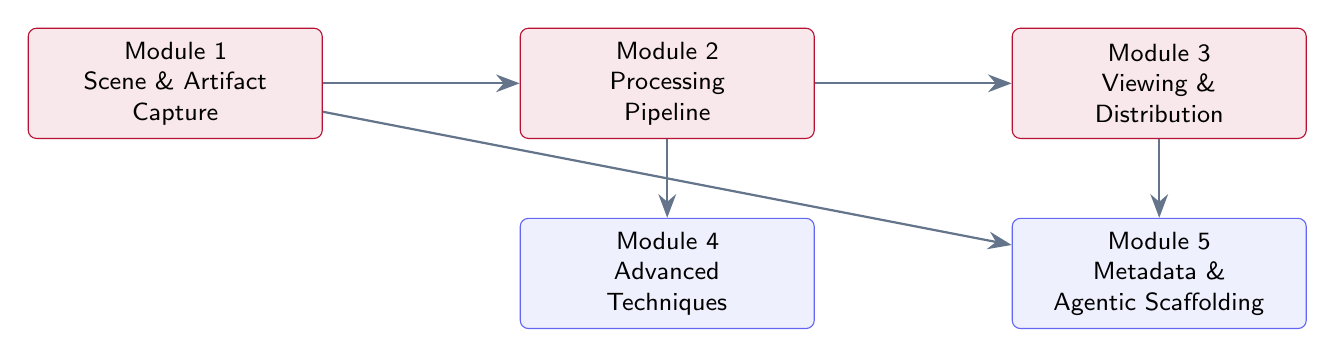
\begin{tikzpicture}[
    node distance=1.8cm and 2.5cm,
    block/.style={
      rectangle, rounded corners=3pt,
      draw=MidGrey, fill=LightGrey,
      text width=3.5cm, minimum height=1.4cm,
      align=center, font=\small\sffamily
    },
    core/.style={block, fill=UoSRed!10, draw=UoSRed},
    advanced/.style={block, fill=DreamLabAccent!10, draw=DreamLabAccent},
    arrow/.style={-{Stealth[length=3mm]}, thick, MidGrey}
  ]
    \node[core] (m1) {Module 1\\Scene \& Artifact\\Capture};
    \node[core, right=of m1] (m2) {Module 2\\Processing\\Pipeline};
    \node[core, right=of m2] (m3) {Module 3\\Viewing \&\\Distribution};
    \node[advanced, below=1cm of m2] (m4) {Module 4\\Advanced\\Techniques};
    \node[advanced, below=1cm of m3] (m5) {Module 5\\Metadata \&\\Agentic Scaffolding};

    \draw[arrow] (m1) -- (m2);
    \draw[arrow] (m2) -- (m3);
    \draw[arrow] (m2) -- (m4);
    \draw[arrow] (m1) -- (m5);
    \draw[arrow] (m3) -- (m5);
  \end{tikzpicture}
  \caption{Module dependency map. Core modules (red border) follow a linear progression; advanced modules (purple border) branch from the core pathway. Module~5 draws on both capture (Module~1) and viewing (Module~3) knowledge.}
  \label{fig:module-map}
\end{figure}

Each module specifies its prerequisites explicitly. Modules~1--3 form the core pathway and should be completed in sequence. Modules~4 and~5 can be taken in either order once their prerequisites are met.

\section{Hardware Tiers}
\label{sec:train-hardware}

Gaussian splat capture and processing spans a wide range of hardware capability and cost. The programme is designed to deliver useful outcomes at every tier, while being transparent about the quality and capability differences between them.

\begin{table}[htbp]
  \centering
  \caption{Hardware tiers for cultural heritage Gaussian splat capture and processing.}
  \label{tab:hardware-tiers}
  \begin{tabular}{@{}L{2.2cm}L{3.5cm}L{3.5cm}L{4cm}@{}}
    \toprule
    \textbf{Tier} & \textbf{Capture Device} & \textbf{Processing} & \textbf{Typical Output} \\
    \midrule
    \textbf{Phone} (Beginner)
      & iPhone 12+ or flagship Android with 4K video, LiDAR optional
      & Cloud processing (Polycam, Luma AI) or institutional GPU server
      & 500K--2M Gaussians, suitable for web viewing \\
    \addlinespace
    \textbf{Consumer Camera} (Intermediate)
      & Mirrorless/DSLR with 4K video (e.g., Sony A7 series, Canon R series), gimbal stabiliser
      & Local workstation with NVIDIA RTX 3080+ (16\,GB VRAM) or institutional GPU server
      & 2M--5M Gaussians, high-quality web and engine viewing \\
    \addlinespace
    \textbf{Professional} (Advanced)
      & Cinema camera (Blackmagic, RED), drone (DJI Mavic/Inspire), terrestrial LiDAR (Leica BLK360)
      & Dedicated GPU workstation with RTX 4090 (24\,GB VRAM) or multi-GPU server
      & 5M--15M Gaussians, archival quality, multi-modal fusion \\
    \bottomrule
  \end{tabular}
\end{table}

\begin{technote}
The phone tier is deliberately included as a first-class pathway. Modern smartphone cameras---particularly the iPhone~15~Pro and Samsung Galaxy S24 Ultra---produce video of sufficient quality for useful Gaussian splat reconstructions. For many cultural heritage scenarios, a phone capture made \emph{today} is infinitely more valuable than a professional capture that never happens due to budget or scheduling constraints.
\end{technote}

\section{Budget Tiers}
\label{sec:train-budget}

Cost is a material constraint for cultural institutions. The programme distinguishes three budget tiers, each with a coherent set of tools that can deliver the full capture-to-viewing workflow:

\begin{table}[htbp]
  \centering
  \caption{Budget tiers for the cultural heritage Gaussian splat workflow.}
  \label{tab:budget-tiers}
  \begin{tabular}{@{}L{2.2cm}L{4cm}L{4cm}L{3cm}@{}}
    \toprule
    \textbf{Tier} & \textbf{Tools} & \textbf{Processing} & \textbf{Monthly Cost} \\
    \midrule
    \textbf{Free}
      & Phone camera, \texttt{gaussian-toolkit} (open source), gsplat.js viewer
      & Institutional GPU server or Google Colab (free tier, limited)
      & \pounds 0 \\
    \addlinespace
    \textbf{Standard} (\pounds 100/month)
      & Consumer camera + gimbal, \texttt{gaussian-toolkit}, cloud GPU (RunPod, Vast.ai)
      & 10--20 captures/month on rented GPU at \pounds 1--3/hour
      & \pounds 50--100 \\
    \addlinespace
    \textbf{Professional} (\pounds 500/month)
      & Professional camera/drone, \texttt{gaussian-toolkit} + SAM3 segmentation, Hunyuan MV API credits, dedicated cloud GPU or on-premises workstation
      & 50+ captures/month, advanced segmentation and inpainting
      & \pounds 300--500 \\
    \bottomrule
  \end{tabular}
\end{table}

\begin{recommendation}
Institutions beginning their Gaussian splat preservation programme should start at the Free tier using existing smartphone hardware and an institutional GPU server. The quality is sufficient for initial cataloguing and public engagement, and early captures establish institutional knowledge that improves the return on investment when upgrading to higher tiers.
\end{recommendation}

\section{Learning Outcomes}
\label{sec:train-outcomes}

Upon completing the full programme, participants will be able to:

\begin{enumerate}
  \item Plan and execute a video capture session optimised for Gaussian splat reconstruction, including camera movement, lighting assessment, and scale reference placement.

  \item Document captures using the structured metadata schema (Module~5), ensuring that technical, curatorial, and rights information accompanies every digital artefact.

  \item Process captured video through the \texttt{gaussian-toolkit} pipeline, from Docker installation through \acrshort{colmap} registration to trained Gaussian splat output.

  \item Evaluate reconstruction quality by inspecting \acrshort{colmap} registration rates, Gaussian count, and visual fidelity in the browser viewer.

  \item Publish Gaussian splat artefacts to web-based viewers and embed them within institutional web pages and collection management systems.

  \item (Advanced) Perform per-object segmentation, scene cleanup, multi-view generation, and game-engine import.

  \item (Advanced) Design and implement automated cataloguing workflows using the agentic metadata scaffolding described in Module~5.
\end{enumerate}

Individual module learning outcomes are specified at the start of each module chapter.

\section{Delivery Format}
\label{sec:train-delivery}

The programme is designed for flexible delivery across multiple formats:

\begin{description}
  \item[Intensive workshop (2--3 days)] All five modules delivered sequentially with hands-on exercises. Requires access to a venue with Wi-Fi, power, and ideally an on-site GPU workstation or cloud GPU allocation. Participants capture a real space on Day~1 and view their processed result on Day~2 or~3.

  \item[Module-per-session (5 half-days)] Each module delivered as a standalone half-day session, typically spaced one or two weeks apart. Allows time for participants to practice between sessions and brings captures from their own contexts.

  \item[Self-directed online] Module materials, video walkthroughs, and exercise specifications provided for asynchronous completion. Requires participants to have access to hardware and processing infrastructure independently.

  \item[Embedded curriculum] Individual modules integrated into existing academic courses in digital media, cultural studies, museum studies, or computer science. Module~1 (Capture) is particularly well-suited to practical studio modules; Module~5 (Metadata) integrates naturally with information science and cataloguing courses.
\end{description}

\begin{keyfinding}
The most effective delivery format observed during the pilot was the intensive workshop, where participants captured a real space on the first day and viewed their reconstructed scene in a browser by the end of the programme. The tangible, immediate result---walking through a digital version of a space they had filmed hours earlier---produced a level of engagement and understanding that no amount of slides or documentation could achieve.
\end{keyfinding}

\chapter{Module 1: Scene and Artifact Capture}
\label{ch:module-capture}

\begin{tcolorbox}[
  enhanced,
  colback=LightGrey,
  colframe=MidGrey,
  fonttitle=\bfseries\sffamily,
  title={Module Information},
  sharp corners=south,
  boxrule=0.6pt
]
\begin{description}[font=\sffamily\bfseries, leftmargin=4cm, style=sameline]
  \item[Prerequisites] None (entry-level module)
  \item[Duration] 3--4 hours (half day)
  \item[Hardware] Any device capable of recording 4K video (smartphone minimum)
  \item[Software] None required for capture; video playback software for review
  \item[Budget tier] Free
\end{description}
\end{tcolorbox}

\medskip

\noindent\textbf{Learning Objectives.} Upon completing this module, participants will be able to:
\begin{enumerate}
  \item Explain why camera movement technique is the dominant quality factor in Gaussian splat reconstruction.
  \item Execute three fundamental capture patterns---orbit, walkthrough, and detail pass---for different scene types.
  \item Assess and manage lighting conditions in gallery, studio, and outdoor capture environments.
  \item Record comprehensive metadata alongside every capture using the structured documentation template.
  \item Evaluate their own captured footage against the quality checklist before submission for processing.
\end{enumerate}

\section{Why Capture Technique Matters}
\label{sec:cap-why}

The experimental results presented in Chapter~\ref{ch:results} demonstrate unambiguously that capture quality is the single most important determinant of reconstruction fidelity. The \acrshort{colmap} \acrlong{sfm} stage (Section~\ref{sec:tech-sfm}) must successfully register a high proportion of extracted frames---ideally above 90\%---to produce a dense, well-distributed point cloud from which Gaussians can be initialised. Poor capture technique leads to failed registrations, sparse point clouds, and reconstructions with holes, floaters, and geometric distortion.

\begin{keyfinding}
In our experimental evaluations, the difference in reconstruction quality between a well-executed phone capture and a poorly executed professional camera capture consistently favoured the phone. Technique dominates equipment.
\end{keyfinding}

The three failure modes most commonly caused by poor capture are:

\begin{enumerate}
  \item \textbf{Registration failure.} Rapid camera movement, motion blur, or insufficient overlap between consecutive frames causes \acrshort{colmap} to fail to match features, leaving unregistered frames and gaps in the reconstruction.

  \item \textbf{Geometric distortion.} Capturing from a narrow range of viewpoints (e.g., only from one side of a room) produces a reconstruction that appears correct from the captured angles but is distorted or hollow when viewed from novel positions.

  \item \textbf{Floaters and artefacts.} Inconsistent lighting, reflective surfaces, or moving objects in the scene produce spurious Gaussians---``floaters''---that appear as ghostly blobs suspended in mid-air when viewing the reconstruction.
\end{enumerate}

\section{Camera Movement Techniques}
\label{sec:cap-movement}

Three fundamental capture patterns cover the majority of cultural heritage scenarios. Most real captures combine two or all three patterns in a single recording session.

\subsection{The Orbit}
\label{sec:cap-orbit}

The orbit is the primary pattern for individual artefacts: sculptures, display cases, small installations, and architectural features. The operator walks in a circle around the subject, maintaining a roughly constant distance and keeping the subject centred in the frame throughout.

\begin{description}
  \item[Movement] Walk slowly and smoothly in a circle around the subject. Maintain a consistent walking pace---approximately half your normal walking speed. Do not stop and start.
  \item[Distance] Stay at a distance of 1--3 metres from the subject. Closer produces higher detail but requires more orbits at different heights to cover the full surface.
  \item[Height variation] Complete a minimum of two orbits: one at the subject's mid-height and one elevated (holding the camera above head height, angled downward). For tall subjects, add a third orbit at a lower angle.
  \item[Duration] A complete orbit set (two heights) for a human-scale subject takes approximately 2--3 minutes of continuous video.
  \item[Overlap] Adjacent frames must share at least 60\% of their visible content. At 30\,fps and a slow walking pace, this is achieved automatically. At 60\,fps, even generous overlap is ensured.
\end{description}

\begin{technote}
The orbit is effective because it provides dense, evenly distributed viewpoints with high inter-frame overlap---exactly what \acrshort{colmap} requires for robust feature matching. The circular trajectory also ensures that every surface is observed from multiple angles, enabling accurate depth estimation.
\end{technote}

\subsection{The Walkthrough}
\label{sec:cap-walkthrough}

The walkthrough is the primary pattern for interior spaces: gallery rooms, exhibition halls, studio spaces, and architectural interiors. The operator walks through the space following a systematic path that covers all areas.

\begin{description}
  \item[Movement] Walk at half normal pace in a serpentine pattern, moving across the room in parallel passes approximately 2--3 metres apart. At each end of the room, turn slowly (do not snap the camera around) and begin the next pass.
  \item[Camera orientation] Angle the camera slightly downward (approximately 10--15 degrees below horizontal) to capture both the walls and the floor. The floor provides critical feature matching points for \acrshort{colmap}---plain, featureless floors are the most common cause of registration failure in interior captures.
  \item[Coverage] After completing the serpentine passes, walk the perimeter of the room close to the walls, capturing wall-mounted works and architectural detail.
  \item[Duration] A typical gallery room (10$\times$10\,m) requires 5--8 minutes of continuous video for thorough coverage.
\end{description}

\begin{recommendation}
If the floor is plain and featureless (polished concrete, white tile), place temporary markers---sheets of printed newspaper, colourful tape crosses, or purpose-printed feature targets---at regular intervals before capture. These provide the visual features that \acrshort{colmap} needs to match frames. The markers can be edited out of the reconstruction later using the inpainting techniques described in Module~4 (Chapter~\ref{ch:module-advanced}).
\end{recommendation}

\subsection{The Detail Pass}
\label{sec:cap-detail}

The detail pass supplements orbit or walkthrough captures with close-up footage of specific features: plaques, textures, fine details, damage or patina, and any elements of particular curatorial interest.

\begin{description}
  \item[Movement] Approach the feature slowly, moving from a medium distance to close-up. Once at close range, orbit the feature with small, slow movements. Then retreat slowly.
  \item[Continuity] The detail pass \emph{must} begin and end with the subject visible at the same distance as the broader orbit or walkthrough footage. This provides the overlap that \acrshort{colmap} needs to register the close-up frames within the broader reconstruction.
  \item[Duration] 30--60 seconds per detail feature.
\end{description}

\begin{technote}
The approach-and-retreat pattern is critical. If you simply film a close-up of a plaque without transitioning from the broader scene, \acrshort{colmap} will be unable to determine where the close-up frames fit within the global reconstruction, and they will be discarded as unregistered frames.
\end{technote}

\section{Lighting Considerations}
\label{sec:cap-lighting}

Lighting is the second most important factor after camera movement. \acrshort{3dgs} is trained against photometric loss---it learns to reproduce the appearance of the scene as observed from the training viewpoints. If the lighting changes between frames (moving clouds, flickering fluorescents, a window that alternates between sun and shadow), the training process receives contradictory signals and produces artefacts.

\subsection{Gallery and Museum Spaces}

Most gallery spaces have controlled, consistent artificial lighting---which is ideal for capture. Key considerations:

\begin{itemize}
  \item \textbf{Avoid mixed lighting zones.} If a gallery has both artificial lighting and natural light from windows, the natural light will change over the course of the capture. Either close blinds/curtains or capture quickly enough that the natural light does not shift appreciably.
  \item \textbf{Spot-lit artworks.} Directional spotlights create strong specular highlights that vary with viewing angle. This is inherently handled by \acrshort{3dgs} through its spherical harmonic colour model, but extremely bright specular reflections (chrome surfaces, glass cases) can still cause artefacts. Capture these areas from more viewpoints than usual to give the training process more data to resolve the view-dependent appearance.
  \item \textbf{Do not use flash.} Flash illumination changes with every frame and is incompatible with photogrammetric reconstruction.
  \item \textbf{Dark spaces.} Some immersive installations deliberately use low light. Increase ISO sensitivity on the camera, accept higher noise, and capture more slowly. Modern denoisers (applied before or during frame extraction) can mitigate noise. Reconstruction quality will be lower than in well-lit spaces, but a noisy capture of a dark installation is still far more useful than no capture at all.
\end{itemize}

\subsection{Outdoor and Site-Specific Locations}

Outdoor captures introduce additional challenges:

\begin{itemize}
  \item \textbf{Overcast days are ideal.} Diffuse cloud cover provides even, consistent illumination without hard shadows. Avoid midday sun, which creates harsh shadows that change as you move around the subject.
  \item \textbf{Avoid golden hour for photogrammetry.} While golden hour light is beautiful for photography, the rapidly changing light direction and colour temperature during sunset/sunrise makes it problematic for multi-minute captures.
  \item \textbf{Moving elements.} Trees, flags, water, and people will create artefacts. Wait for still moments if possible, or plan to use masking and cleanup in post-processing (Module~4).
\end{itemize}

\section{Metadata Documentation}
\label{sec:cap-metadata}

Every capture must be accompanied by a structured metadata record. This is not optional overhead---it is an integral part of the preservation workflow. A 3D reconstruction without metadata is an orphaned file; with metadata, it is a cultural heritage record.

The full metadata schema is defined in Module~5 (Chapter~\ref{ch:module-metadata}). At the point of capture, the operator must record the following information, using either the printed field sheet or the digital form provided:

\subsection{Required Fields}

\begin{description}
  \item[Scene title] A descriptive title for the capture (e.g., ``Main Gallery, North Wall Installation'').
  \item[Date and time] ISO~8601 format: \texttt{2026-04-01T14:30:00Z}. The time is important for correlating with lighting conditions.
  \item[Location] Venue name and, for outdoor captures, GPS coordinates. Modern smartphones record GPS in video metadata automatically; for cameras without GPS, use a phone to note coordinates.
  \item[Creator/artist credits] The name(s) of the artist(s) or creator(s) whose work appears in the capture. For gallery spaces containing multiple works, list all.
  \item[Capture operator] Who performed the capture.
  \item[Rights and permissions] Under what licence or permission the capture was made. Note any restrictions on distribution, commercial use, or public display.
  \item[Material descriptions] A brief description of the physical materials present: ``wire mesh sculpture, approximately 2\,m tall, mixed media including found objects and LED lighting.''
  \item[Lighting conditions] General lighting description: ``artificial gallery track lighting, no natural light, even illumination'' or ``mixed natural (skylights) and artificial (spot), afternoon.''
  \item[Scale reference] Whether a scale reference (ruler, known-size object) is visible in the capture. If so, describe its location and size.
  \item[Cultural context notes] Any contextual information that a future viewer would need to understand the work: its place in an exhibition, relationship to other works, artist's intent, historical significance.
\end{description}

\subsection{Agentic Scaffolding: The Capture Metadata Record}
\label{sec:cap-agentic}

The metadata fields above are formalised as a JSON schema that serves dual purposes: human documentation and machine processing. When the operator completes the capture form (either on paper or digitally), the information is structured into the following format for ingestion by the agentic pipeline described in Chapter~\ref{ch:pipeline}:

\begin{lstlisting}[language={}, caption={Capture-time metadata record (JSON).}, label={lst:capture-metadata}]
{
  "capture": {
    "id": "auto-generated UUID",
    "title": "Main Gallery, North Wall Installation",
    "date": "2026-04-01T14:30:00Z",
    "location": {
      "name": "University of Salford, New Adelphi Gallery",
      "gps": [53.4870, -2.2742]
    },
    "creator": "Artist Name",
    "operator": "Capture Operator Name",
    "rights": "CC BY-SA 4.0",
    "description": "Wire mesh figure, 2m tall, mixed media",
    "lighting": "artificial gallery track, even",
    "scale_reference": "30cm ruler on plinth base",
    "cultural_context": "Part of 'Material Worlds' exhibition,
                          Spring 2026"
  },
  "technical": {
    "device": "iPhone 15 Pro",
    "resolution": "4K (3840x2160)",
    "fps": 30,
    "duration_seconds": 180,
    "stabilisation": "handheld",
    "capture_pattern": ["orbit", "detail_pass"]
  }
}
\end{lstlisting}

This record is stored alongside the video file and accompanies it through the processing pipeline, where the agentic orchestrator appends processing results (Chapter~\ref{ch:module-metadata}).

\section{Practical Exercise: Capture a Room in Your Building}
\label{sec:cap-exercise}

\begin{tcolorbox}[
  enhanced,
  colback=SuccessGreen!8,
  colframe=SuccessGreen,
  fonttitle=\bfseries\sffamily,
  title={Exercise 1.1: Room Capture},
  sharp corners=south,
  boxrule=0.6pt
]
\textbf{Objective:} Capture a room or space in your building that could plausibly be a cultural heritage preservation target.

\textbf{Time:} 45--60 minutes (including preparation and metadata)

\textbf{Equipment:} Smartphone with 4K video capability

\textbf{Steps:}
\begin{enumerate}
  \item \textbf{Scout the space} (10 minutes). Walk through the room without filming. Identify: lighting conditions, reflective surfaces, featureless areas (plain walls, floors), moving elements (people, screens), and features of particular interest.
  \item \textbf{Plan your capture path} (5 minutes). Sketch the room on paper and draw your planned walkthrough serpentine path, noting where you will perform detail passes.
  \item \textbf{Prepare the space.} If the floor is featureless, place newspaper sheets or tape crosses at 2\,m intervals. Remove or note any moving elements.
  \item \textbf{Complete the metadata form} (5 minutes). Fill in all required fields from Section~\ref{sec:cap-metadata}.
  \item \textbf{Record the walkthrough} (5--8 minutes of continuous video). Follow your planned path at half walking speed. Do not stop, do not adjust the camera mid-recording, and do not use zoom.
  \item \textbf{Record detail passes} (2--5 minutes). Select 2--3 features of interest and perform the approach--orbit--retreat pattern for each.
  \item \textbf{Review your footage.} Play back on your phone. Check for: consistent framing, absence of motion blur, sufficient coverage of all walls and the floor.
\end{enumerate}

\textbf{Expected outcome:} 7--13 minutes of continuous 4K video, a completed metadata form, and a hand-drawn capture plan. This footage will be processed in Module~2 (Chapter~\ref{ch:module-processing}).
\end{tcolorbox}

\section{Quality Checklist}
\label{sec:cap-checklist}

Before submitting footage for processing, verify each of the following. A failure on any item marked \textbf{Critical} is likely to cause processing failure or severe quality degradation.

\begin{table}[htbp]
  \centering
  \caption{Pre-submission quality checklist for captured footage.}
  \label{tab:capture-checklist}
  \begin{tabular}{@{}l L{8cm} l@{}}
    \toprule
    \textbf{Priority} & \textbf{Check} & \textbf{Remedy} \\
    \midrule
    Critical & Video is in 4K resolution (3840$\times$2160 or higher) & Recapture \\
    Critical & No motion blur visible when pausing at random frames & Recapture more slowly \\
    Critical & Continuous recording (no cuts, pauses, or zoom changes) & Recapture \\
    Critical & Camera moved smoothly throughout (no sudden jerks) & Recapture \\
    \addlinespace
    Important & All surfaces captured from at least two distinct angles & Add supplementary passes \\
    Important & Floor/ground visible in walkthrough frames & Recapture with camera angled down \\
    Important & Scale reference visible in at least one section & Place ruler and add detail pass \\
    Important & Consistent lighting throughout capture duration & Close blinds or recapture \\
    \addlinespace
    Desirable & Multiple height levels captured in orbits & Add elevated orbit pass \\
    Desirable & No people or moving objects in frame & Recapture or note for post cleanup \\
    Desirable & Detail passes for all features of curatorial interest & Add detail passes \\
    \bottomrule
  \end{tabular}
\end{table}

\begin{keyfinding}
The checklist above encodes the most common failure modes observed during the pilot project. Approximately 70\% of processing failures were traceable to one of the four ``Critical'' items. Making the checklist a mandatory pre-submission step eliminates the most expensive failures---those that consume GPU processing time before failing.
\end{keyfinding}

\chapter{Module 2: Processing Pipeline}
\label{ch:module-processing}

\begin{tcolorbox}[
  enhanced,
  colback=LightGrey,
  colframe=MidGrey,
  fonttitle=\bfseries\sffamily,
  title={Module Information},
  sharp corners=south,
  boxrule=0.6pt
]
\begin{description}[font=\sffamily\bfseries, leftmargin=4cm, style=sameline]
  \item[Prerequisites] Module~1 (Chapter~\ref{ch:module-capture}); basic comfort with command-line interfaces
  \item[Duration] 4--6 hours (including processing wait time)
  \item[Hardware] Computer with NVIDIA GPU (8\,GB+ VRAM), or access to a cloud GPU instance
  \item[Software] Docker Desktop, web browser, terminal emulator
  \item[Budget tier] Free (with institutional GPU) or Standard (\pounds 1--3/hour cloud GPU)
\end{description}
\end{tcolorbox}

\medskip

\noindent\textbf{Learning Objectives.} Upon completing this module, participants will be able to:
\begin{enumerate}
  \item Install Docker and the \texttt{gaussian-toolkit} on a local workstation or cloud GPU instance.
  \item Upload captured video to the pipeline's web interface and initiate processing.
  \item Monitor pipeline progress through each stage (\acrshort{colmap}, training, optional mesh extraction).
  \item Interpret the key quality indicators in the pipeline output.
  \item Identify and resolve the five most common processing failures.
  \item Access and navigate the reconstructed scene in the built-in browser viewer.
\end{enumerate}

\section{Installing Docker and the Gaussian Toolkit}
\label{sec:proc-install}

The \texttt{gaussian-toolkit} is distributed as a set of Docker containers, as described in Chapter~\ref{ch:pipeline}. This eliminates the need to install CUDA, Python, \acrshort{colmap}, or any of the other GPU-accelerated dependencies manually---a process that, in our experience, takes even experienced developers 4--8 hours and is the single most common point of abandonment for new users of 3D reconstruction tools.

\subsection{Prerequisites}

Before beginning installation, verify that your system meets the following requirements:

\begin{itemize}
  \item \textbf{Operating system:} Linux (Ubuntu 20.04+), Windows 10/11 with WSL2, or macOS (CPU-only, significantly slower).
  \item \textbf{GPU:} NVIDIA GPU with 8\,GB+ VRAM and CUDA compute capability 7.0 or higher. The RTX 3060 (12\,GB) is the minimum recommended for practical use; the RTX 3080/4070 (16\,GB) or above is recommended for comfortable operation.
  \item \textbf{Disk space:} At least 50\,GB free for Docker images and working data.
  \item \textbf{RAM:} 16\,GB minimum, 32\,GB recommended.
  \item \textbf{Docker:} Docker Desktop (Windows/macOS) or Docker Engine (Linux), version 24.0 or later.
  \item \textbf{NVIDIA Container Toolkit:} Required on Linux; included in Docker Desktop for Windows with WSL2.
\end{itemize}

\subsection{Installation Steps}

\begin{lstlisting}[language=bash, caption={Installing the \texttt{gaussian-toolkit}.}, label={lst:install}]
# 1. Clone the repository
git clone https://github.com/dreamlab-ai/gaussian-toolkit.git
cd gaussian-toolkit

# 2. Pull the pre-built Docker images (approximately 30 GB)
docker compose pull

# 3. Start the services
docker compose up -d

# 4. Verify all services are running
docker compose ps

# 5. Open the web interface
# Navigate to http://localhost:8080 in your browser
\end{lstlisting}

\begin{technote}
The initial \texttt{docker compose pull} downloads approximately 30\,GB of container images. On a typical university network connection (100\,Mbps), this takes 30--45 minutes. Subsequent starts are near-instant as images are cached locally. For workshop delivery, pre-pulling images on all participant machines before the session begins is strongly recommended.
\end{technote}

\subsection{Cloud GPU Alternative}

For participants without local GPU access, cloud GPU instances provide an accessible alternative. The following providers have been tested with the \texttt{gaussian-toolkit}:

\begin{table}[htbp]
  \centering
  \caption{Cloud GPU options for \texttt{gaussian-toolkit} processing.}
  \label{tab:cloud-gpu}
  \begin{tabular}{@{}L{2.5cm}L{3cm}L{2.5cm}L{2cm}L{2.5cm}@{}}
    \toprule
    \textbf{Provider} & \textbf{GPU} & \textbf{VRAM} & \textbf{Cost/hr} & \textbf{Notes} \\
    \midrule
    RunPod       & RTX 4090     & 24\,GB & \$0.44 & Docker-native \\
    Vast.ai      & RTX 3090     & 24\,GB & \$0.25 & Variable pricing \\
    Lambda Labs  & A10G         & 24\,GB & \$0.60 & Persistent instances \\
    Google Colab & T4 (free) / A100 (Pro) & 16/40\,GB & \$0--12/mo & Notebook interface \\
    \bottomrule
  \end{tabular}
\end{table}

For cloud deployment, the \texttt{gaussian-toolkit} provides a one-command setup script:

\begin{lstlisting}[language=bash, caption={Cloud instance quick setup.}, label={lst:cloud-setup}]
# On a fresh cloud GPU instance (Ubuntu + NVIDIA drivers)
curl -fsSL https://get.docker.com | sh
sudo nvidia-ctk runtime configure --runtime=docker
sudo systemctl restart docker
git clone https://github.com/dreamlab-ai/gaussian-toolkit.git
cd gaussian-toolkit && docker compose up -d
\end{lstlisting}

\section{Uploading Video to the Web Interface}
\label{sec:proc-upload}

The \texttt{gaussian-toolkit} web interface provides a drag-and-drop upload mechanism accessible at \texttt{http://localhost:8080} (local) or the cloud instance's public IP address.

\subsection{Upload Process}

\begin{enumerate}
  \item Open the web interface in a browser (Chrome or Firefox recommended).
  \item Click \textbf{New Project} and enter a descriptive project name (e.g., ``North Gallery 2026-04-01'').
  \item Drag the captured video file onto the upload area, or click to browse. Supported formats: MP4 (H.264/H.265), MOV, AVI.
  \item Select the processing configuration:
    \begin{description}
      \item[Quick] 7,000 training iterations, \acrshort{colmap} exhaustive matching. Fastest results (20--40 minutes for a 3-minute video on RTX 4090), lower fidelity.
      \item[Standard] 30,000 iterations, \acrshort{colmap} sequential matching. Recommended for most captures (1--2 hours).
      \item[Archival] 50,000 iterations, \acrshort{colmap} exhaustive matching, all three training variants (\acrshort{3dgs}, \acrshort{mrnf}, \acrshort{mcmc}). Highest fidelity, longest processing time (3--6 hours).
    \end{description}
  \item Optionally enable mesh extraction (TSDF and/or MILo) if mesh outputs are required.
  \item Click \textbf{Start Processing}.
\end{enumerate}

\begin{recommendation}
For training purposes, use the \textbf{Quick} configuration for initial runs. The reduced iteration count produces a visibly lower-fidelity result, but it completes in 20--40 minutes rather than 1--2 hours, allowing participants to iterate on capture technique within a single workshop session. Once the capture technique is validated, reprocess the same footage with the \textbf{Standard} or \textbf{Archival} configuration for the final preservation artefact.
\end{recommendation}

\section{Monitoring the Pipeline}
\label{sec:proc-monitoring}

The web interface provides real-time progress monitoring through a multi-stage status display. Understanding what each stage does, and what constitutes normal versus abnormal behaviour, is essential for troubleshooting.

\subsection{Stage 1: Frame Extraction}

The pipeline extracts frames from the uploaded video using FFmpeg. The interface displays:

\begin{itemize}
  \item \textbf{Total frames extracted.} A 3-minute 4K video at 30\,fps produces approximately 5,400 frames. The pipeline extracts at a configurable rate (default: every second frame, yielding approximately 2,700 frames for a 3-minute video).
  \item \textbf{Frames rejected.} Blurred or near-duplicate frames are discarded by the Laplacian variance filter. A rejection rate above 20\% suggests the camera was moving too fast.
  \item \textbf{Final frame count.} Typically 1,500--3,000 frames for a 3--5 minute capture.
\end{itemize}

\subsection{Stage 2: COLMAP Structure-from-Motion}
\label{sec:proc-colmap}

This is the most time-consuming and failure-prone stage. \acrshort{colmap} processes the extracted frames to determine camera positions and produce a sparse 3D point cloud (see Section~\ref{sec:tech-sfm}).

The interface displays:

\begin{itemize}
  \item \textbf{Feature extraction progress.} Each frame is analysed for distinctive visual features (SIFT descriptors). This is parallelised across CPU cores and completes relatively quickly.
  \item \textbf{Feature matching progress.} Frames are compared pairwise to identify shared features. This is the slowest sub-stage, growing quadratically with frame count for exhaustive matching and linearly for sequential matching.
  \item \textbf{Registered images.} The number of frames successfully placed in 3D space. This is the single most important quality indicator.
  \item \textbf{Registration rate.} Registered images divided by total frames. The target is $\geq 90\%$.
  \item \textbf{Sparse points.} The number of 3D points in the reconstructed sparse cloud. Typical values range from 50,000 to 500,000 depending on scene complexity and capture thoroughness.
\end{itemize}

\begin{keyfinding}
The \acrshort{colmap} registration rate is the earliest and most reliable predictor of final reconstruction quality. A rate below 80\% almost always produces a reconstruction with visible holes or distortion. A rate below 50\% typically indicates a fundamental capture problem (motion blur, insufficient overlap) and the footage should be recaptured rather than reprocessed.
\end{keyfinding}

\subsection{Stage 3: Gaussian Splat Training}

Once \acrshort{colmap} completes, the Gaussian splat training begins. The interface displays:

\begin{itemize}
  \item \textbf{Current iteration} and progress bar (e.g., 15,000/30,000).
  \item \textbf{Training loss.} The photometric error between the rendered Gaussians and the training images. This should decrease rapidly in the first few thousand iterations, then gradually plateau.
  \item \textbf{Gaussian count.} The number of Gaussians in the scene, which increases through densification and decreases through pruning. Typical converged values range from 500,000 to 5,000,000 depending on scene complexity.
  \item \textbf{Preview renders.} Every 1,000 iterations, the interface renders a preview from a fixed viewpoint, allowing participants to watch the reconstruction emerge in real time.
\end{itemize}

\subsection{Stage 4: Mesh Extraction (Optional)}

If mesh extraction was enabled, one or both of the following processes run after training:

\begin{description}
  \item[TSDF fusion] Renders depth maps from the trained Gaussians at each camera position, then fuses them into a volumetric grid that is converted to a triangle mesh via marching cubes. Produces water-tight meshes but may lose fine detail.
  \item[MILo] A learned mesh extraction method that directly converts the Gaussian representation to a triangle mesh using a neural network. Produces higher-detail meshes but requires the MILo sidecar container.
\end{description}

\section{Understanding the Output}
\label{sec:proc-output}

Upon completion, the pipeline produces the following output files, accessible through the web interface's download panel or directly from the Docker volume:

\begin{table}[htbp]
  \centering
  \caption{Pipeline output files and their uses.}
  \label{tab:output-files}
  \begin{tabular}{@{}l l L{6cm}@{}}
    \toprule
    \textbf{File} & \textbf{Format} & \textbf{Use} \\
    \midrule
    \texttt{scene.ply}   & PLY (Gaussian) & The native Gaussian splat representation. Primary preservation artefact. Loadable in browser viewers and Gaussian-aware applications. \\
    \texttt{scene.splat}  & SPLAT binary   & Compressed format for browser viewers (antimatter15/splat, gsplat.js). Faster loading, same visual quality. \\
    \texttt{scene.glb}    & glTF Binary    & Triangle mesh (if mesh extraction enabled). Compatible with Blender, Unreal, Unity, and web-based 3D viewers (model-viewer). \\
    \texttt{scene.usda}   & USD ASCII      & Universal Scene Description (if enabled). The preferred interchange format for production 3D workflows and long-term archival. \\
    \texttt{cameras.json} & JSON           & Camera positions and intrinsics from \acrshort{colmap}. Useful for registering additional captures of the same space. \\
    \texttt{metadata.json} & JSON          & The complete capture and processing metadata record (see Module~5, Chapter~\ref{ch:module-metadata}). \\
    \bottomrule
  \end{tabular}
\end{table}

\begin{technote}
The \texttt{.ply} file containing the Gaussian splat representation is typically 50--200\,MB for a standard scene. The \texttt{.splat} file is a sorted, compressed version at approximately 60\% of the PLY size. The \texttt{.glb} mesh file varies widely---from 10\,MB for a simplified mesh to 500\,MB+ for a high-detail extraction---and contains texture maps baked from the Gaussian representation.
\end{technote}

\section{Viewing Results in the Browser}
\label{sec:proc-viewing}

The pipeline's built-in browser viewer is accessible immediately upon completion at \texttt{http://localhost:8080/viewer/\{project-id\}}. The viewer supports:

\begin{itemize}
  \item \textbf{Orbit navigation.} Click and drag to rotate around the scene centre. Scroll to zoom.
  \item \textbf{Fly-through navigation.} WASD keys for movement, mouse for look direction. This mode allows free exploration of the reconstructed space.
  \item \textbf{Quality comparison.} Toggle between the Gaussian splat and mesh representations (if both were generated) to observe the quality difference first-hand.
  \item \textbf{Gaussian count display.} Shows the number of Gaussians being rendered and the current frame rate. Useful for assessing whether the scene is within the viewer's comfortable rendering budget.
\end{itemize}

\section{Troubleshooting Common Issues}
\label{sec:proc-troubleshoot}

Table~\ref{tab:troubleshoot} documents the five most common processing issues encountered during the pilot project, their symptoms, likely causes, and remedies.

\begin{table}[htbp]
  \centering
  \caption{Common processing issues and remedies.}
  \label{tab:troubleshoot}
  \begin{tabular}{@{}L{2.5cm}L{3cm}L{3cm}L{4cm}@{}}
    \toprule
    \textbf{Symptom} & \textbf{Likely Cause} & \textbf{Evidence} & \textbf{Remedy} \\
    \midrule
    \acrshort{colmap} registration $< 50\%$
      & Motion blur or insufficient frame overlap
      & Blurred frames visible when reviewing extracted images
      & Recapture at slower pace; increase frame extraction rate \\
    \addlinespace
    Large holes in reconstruction
      & Area not captured from enough viewpoints
      & Missing coverage visible in \acrshort{colmap} sparse point cloud
      & Capture additional footage of the missing area and merge \\
    \addlinespace
    Floating blobs (``floaters'')
      & Moving objects in scene or strong reflections
      & Floaters correspond to locations of people, screens, or mirrors
      & Recapture without moving elements; use SAM3 cleanup (Module~4) \\
    \addlinespace
    Out of GPU memory
      & Too many frames or excessively high resolution
      & CUDA out-of-memory error in training logs
      & Reduce frame extraction rate; downsample to 2K; use GPU with more VRAM \\
    \addlinespace
    Pipeline hangs at ``Feature matching''
      & Exhaustive matching on too many frames
      & Matching progress stalls at high frame counts ($>$3,000)
      & Switch to sequential matching mode; reduce frame count \\
    \bottomrule
  \end{tabular}
\end{table}

\section{Practical Exercise: Process Your Captured Video}
\label{sec:proc-exercise}

\begin{tcolorbox}[
  enhanced,
  colback=SuccessGreen!8,
  colframe=SuccessGreen,
  fonttitle=\bfseries\sffamily,
  title={Exercise 2.1: Pipeline Processing},
  sharp corners=south,
  boxrule=0.6pt
]
\textbf{Objective:} Process the video captured in Exercise~1.1 (Section~\ref{sec:cap-exercise}) through the full \texttt{gaussian-toolkit} pipeline.

\textbf{Time:} 30 minutes setup + 20--40 minutes processing (Quick mode) or 1--2 hours (Standard mode)

\textbf{Equipment:} Computer with Docker and \texttt{gaussian-toolkit} installed (per Section~\ref{sec:proc-install}), or cloud GPU instance

\textbf{Steps:}
\begin{enumerate}
  \item Upload your captured video to the web interface and select \textbf{Quick} configuration.
  \item While processing runs, record the following metrics as they appear:
    \begin{itemize}
      \item Total frames extracted: \rule{3cm}{0.4pt}
      \item Frames rejected (blur): \rule{3cm}{0.4pt}
      \item \acrshort{colmap} registration rate: \rule{3cm}{0.4pt}
      \item Sparse points: \rule{3cm}{0.4pt}
      \item Final Gaussian count: \rule{3cm}{0.4pt}
    \end{itemize}
  \item When processing completes, open the browser viewer and navigate through your reconstruction.
  \item Identify and note any quality issues: holes, floaters, distortion, missing areas.
  \item Correlate any quality issues with your capture technique: can you identify what you would do differently?
  \item If your registration rate was below 80\%, recapture and reprocess.
\end{enumerate}

\textbf{Expected outcome:} A viewable Gaussian splat reconstruction of the room captured in Exercise~1.1, accompanied by an understanding of how capture decisions map to reconstruction quality. Participants should be able to articulate at least one specific improvement they would make to their capture technique.
\end{tcolorbox}

\begin{tcolorbox}[
  enhanced,
  colback=SuccessGreen!8,
  colframe=SuccessGreen,
  fonttitle=\bfseries\sffamily,
  title={Exercise 2.2: Quality Comparison},
  sharp corners=south,
  boxrule=0.6pt
]
\textbf{Objective:} Compare Quick and Standard processing of the same footage to understand the quality--time trade-off.

\textbf{Time:} 1--2 hours (processing time for Standard configuration)

\textbf{Steps:}
\begin{enumerate}
  \item Reprocess the same video using the \textbf{Standard} configuration (30,000 iterations).
  \item Open both results in the browser viewer (two tabs) and compare:
    \begin{itemize}
      \item Fine detail (text on labels, surface textures)
      \item Edge sharpness (transitions between objects)
      \item Floaters and artefacts
      \item Overall colour fidelity
    \end{itemize}
  \item Record your observations: is the quality difference worth the additional processing time for this particular scene?
\end{enumerate}

\textbf{Expected outcome:} Participants should observe noticeably finer detail and fewer artefacts in the Standard output, and be able to make an informed decision about which configuration to use for different capture scenarios.
\end{tcolorbox}

\chapter{Module 3: Viewing and Distribution}
\label{ch:module-viewing}

\begin{tcolorbox}[
  enhanced,
  colback=LightGrey,
  colframe=MidGrey,
  fonttitle=\bfseries\sffamily,
  title={Module Information},
  sharp corners=south,
  boxrule=0.6pt
]
\begin{description}[font=\sffamily\bfseries, leftmargin=4cm, style=sameline]
  \item[Prerequisites] Module~2 (Chapter~\ref{ch:module-processing}); basic HTML/web knowledge helpful but not required
  \item[Duration] 3--4 hours (half day)
  \item[Hardware] Any computer with a modern web browser (Chrome 113+, Firefox 114+, Edge 113+)
  \item[Software] Text editor; optionally Blender 4.0+ or Unreal Engine 5.4+
  \item[Budget tier] Free
\end{description}
\end{tcolorbox}

\medskip

\noindent\textbf{Learning Objectives.} Upon completing this module, participants will be able to:
\begin{enumerate}
  \item Load and navigate a Gaussian splat scene in two or more browser-based viewers.
  \item Embed a splat viewer within an existing web page using an \texttt{<iframe>} element.
  \item Explain the trade-offs between WebGL and WebGPU rendering paths for splat viewers.
  \item Import Gaussian splat and mesh outputs into Unreal Engine~5.4+ for immersive experiences.
  \item Identify appropriate archival formats and implement a basic preservation strategy for 3D captures.
  \item Embed descriptive metadata within a \acrshort{usd} scene file.
\end{enumerate}

\section{Browser-Based Splat Viewers}
\label{sec:view-browser}

Browser-based viewing is the primary delivery mechanism recommended by this report (Chapter~\ref{ch:recommendations}). It requires no software installation, no specialised hardware, and no technical expertise from the audience. A Gaussian splat scene viewed in a browser is as accessible as a YouTube video---and considerably more interactive.

Several open-source viewer implementations are available, each with different capabilities and trade-offs. Table~\ref{tab:viewer-detail} extends the comparison introduced in Chapter~\ref{ch:recommendations} with implementation detail relevant to deployment decisions.

\begin{table}[htbp]
  \centering
  \caption{Browser-based splat viewer comparison (extended).}
  \label{tab:viewer-detail}
  \begin{tabular}{@{}L{2.5cm}L{3cm}L{3cm}L{4cm}@{}}
    \toprule
    \textbf{Viewer} & \textbf{Rendering} & \textbf{Input Format} & \textbf{Key Characteristics} \\
    \midrule
    gsplat.js
      & WebGL2 + WebGPU
      & \texttt{.ply}, \texttt{.splat}
      & Most feature-rich open-source option. Supports progressive loading, level-of-detail, and custom shading. Active development. MIT licence. \\
    \addlinespace
    antimatter15/splat
      & WebGL2
      & \texttt{.splat}
      & Lightweight, minimal dependencies. Excellent mobile performance. Good choice for embedding where simplicity is prioritised. MIT licence. \\
    \addlinespace
    gaussian-toolkit viewer
      & WebGL2
      & \texttt{.ply}, \texttt{.splat}
      & Integrated with the processing pipeline. Includes metadata overlay, quality comparison mode, and measurement tools. MIT licence. \\
    \addlinespace
    Luma AI viewer
      & WebGPU
      & Proprietary
      & Highest rendering quality. Requires uploading data to Luma's servers. Not self-hostable. Free tier available. \\
    \addlinespace
    PlayCanvas
      & WebGL2 + WebGPU
      & \texttt{.ply}
      & Full 3D engine with splat support. Suitable when splats need to be integrated with other 3D content (annotations, UI overlays). MIT licence. \\
    \bottomrule
  \end{tabular}
\end{table}

\begin{recommendation}
For institutional deployment where data sovereignty and long-term availability are requirements, use a self-hosted viewer (gsplat.js, antimatter15/splat, or the \texttt{gaussian-toolkit} viewer). Cloud-hosted viewers may change their terms of service, introduce paywalls, or discontinue service. Cultural heritage artefacts must be accessible on timescales measured in decades, not product cycles.
\end{recommendation}

\subsection{Loading a Scene in gsplat.js}

The gsplat.js viewer can be deployed as a static web page with no server-side components. The minimal deployment requires three files:

\begin{lstlisting}[language=HTML, caption={Minimal gsplat.js viewer deployment.}, label={lst:gsplat-viewer}]
<!DOCTYPE html>
<html>
<head>
  <title>Cultural Heritage Viewer</title>
  <style>
    body { margin: 0; overflow: hidden; }
    canvas { width: 100vw; height: 100vh; }
  </style>
</head>
<body>
  <canvas id="viewer"></canvas>
  <script type="module">
    import { Viewer } from 'https://cdn.jsdelivr.net/npm/gsplat@latest';

    const viewer = new Viewer({
      canvas: document.getElementById('viewer'),
      url: './scene.splat'
    });
  </script>
</body>
</html>
\end{lstlisting}

\begin{technote}
The \texttt{.splat} file format used by browser viewers is a sorted, compressed binary encoding of the Gaussian parameters optimised for progressive loading. The viewer begins rendering as soon as the first chunk of data arrives, providing a coarse representation that progressively refines as more Gaussians load. A 100\,MB splat file typically begins rendering within 2--3 seconds on a standard broadband connection.
\end{technote}

\subsection{Loading a Scene in antimatter15/splat}

The antimatter15 viewer is even more minimal, consisting of a single HTML file:

\begin{lstlisting}[language=bash, caption={Deploying the antimatter15 splat viewer.}, label={lst:antimatter-deploy}]
# Clone the viewer
git clone https://github.com/antimatter15/splat.git
cd splat

# Copy your .splat file to the viewer directory
cp /path/to/scene.splat ./

# Serve locally (any HTTP server works)
python3 -m http.server 8000

# Open http://localhost:8000 in browser
# Drag and drop scene.splat onto the page
\end{lstlisting}

\section{Embedding in Websites}
\label{sec:view-embed}

For institutional deployment, Gaussian splat viewers are most commonly embedded within existing web pages---collection catalogue entries, exhibition documentation pages, or standalone heritage portals---using HTML \texttt{<iframe>} elements.

\subsection{Basic Embedding}

\begin{lstlisting}[language=HTML, caption={Embedding a splat viewer in an existing web page.}, label={lst:embed-iframe}]
<div class="heritage-viewer" style="width:100%; max-width:1200px;">
  <iframe
    src="https://heritage.salford.ac.uk/viewer/north-gallery-2026"
    width="100%"
    height="600"
    frameborder="0"
    allow="fullscreen; xr-spatial-tracking"
    loading="lazy"
    title="3D reconstruction of North Gallery, April 2026">
  </iframe>
  <p class="caption">
    <strong>North Gallery Installation</strong> by Artist Name,
    captured 1 April 2026.
    <a href="/catalogue/NG-2026-001">View catalogue record</a>.
  </p>
</div>
\end{lstlisting}

Key attributes for accessibility and performance:

\begin{description}
  \item[\texttt{loading="lazy"}] Defers loading the viewer until it scrolls into the viewport, preventing heavy 3D scenes from blocking page load.
  \item[\texttt{title}] Provides an accessible description for screen readers. Since splat viewers are inherently visual, the title should describe the content for users who cannot see the 3D scene.
  \item[\texttt{allow="fullscreen; xr-spatial-tracking"}] Enables fullscreen mode and, where supported, WebXR passthrough for AR viewing on compatible devices.
\end{description}

\subsection{Integration with Collection Management Systems}

Most institutional collection management systems (CMS) support custom content types or embed blocks. The specific integration depends on the CMS in use:

\begin{description}
  \item[CollectiveAccess] Add a custom media representation type for Gaussian splats. Configure the ``3D viewer'' display to embed the viewer iframe using the splat file URL stored as a media field.
  \item[Omeka S] Use the Omeka ``iframe embed'' module or a custom block layout to embed the viewer. Associate the splat file and its metadata JSON as media items on the catalogue record.
  \item[WordPress (institutional sites)] Use the standard HTML block or a custom shortcode to embed the iframe. Store the \texttt{.splat} file in the media library or on a CDN.
  \item[Custom systems] Expose the viewer as a standalone page (one per capture) behind the institution's authentication and serve the iframe URL as a field in the catalogue database.
\end{description}

\section{Unreal Engine Import}
\label{sec:view-unreal}

For high-fidelity immersive experiences---VR installations, exhibition kiosks, and research visualisation---Unreal Engine~5.4 and later provides native Gaussian splat rendering through community and commercial plugins.

\subsection{Plugin Options}

\begin{description}
  \item[3D Gaussian Splatting for UE5 (Luma AI)] Free plugin supporting direct import of \texttt{.ply} Gaussian splat files. Renders using the engine's deferred rendering pipeline with support for shadows, post-processing, and VR stereo rendering.
  \item[GaussianSplattingUE (community)] Open-source plugin with editor integration, allowing splats to be placed, scaled, and lit within standard Unreal scenes alongside conventional meshes and materials.
  \item[Cesium for Unreal + 3D Tiles] For geospatially-referenced captures (outdoor heritage sites, building exteriors), the Cesium plugin can stream splat data as 3D Tiles, enabling integration with geospatial datasets, satellite imagery, and other site data.
\end{description}

\subsection{Import Workflow}

\begin{enumerate}
  \item Install the chosen plugin from the Unreal Marketplace or GitHub.
  \item Import the \texttt{scene.ply} file into the Unreal content browser. The plugin converts it to an internal Gaussian splat asset.
  \item Drag the asset into the level viewport. Position and scale it using the standard transform gizmo.
  \item Configure rendering parameters: splat size multiplier, near/far clip planes, maximum Gaussian count for performance budget.
  \item For VR deployment, enable stereo rendering in the plugin settings and test with a connected headset.
\end{enumerate}

\begin{technote}
Unreal Engine renders Gaussian splats using a custom render pass that integrates with the engine's depth buffer but not its material system. This means splats receive post-processing effects (bloom, tone mapping, ambient occlusion) but cannot have Unreal materials applied to them. For scenes that mix splats with conventional meshes, careful attention to lighting and colour grading is needed to maintain visual consistency.
\end{technote}

\section{VR and AR Viewing Options}
\label{sec:view-xr}

Volumetric cultural heritage content is particularly compelling in virtual and augmented reality, where the spatial qualities of the original work can be experienced with natural head movement and stereo depth perception.

\begin{description}
  \item[VR headsets (Meta Quest 3, Apple Vision Pro, PCVR)] Unreal Engine with a Gaussian splat plugin provides the highest-quality VR experience. For standalone headsets (Quest 3), WebXR-enabled browser viewers offer a zero-install pathway, though at lower quality and frame rate than native rendering.

  \item[AR on mobile devices] WebXR-capable browsers (Chrome for Android, Safari for iOS 17+) can overlay Gaussian splat scenes onto the real world using the device camera. This enables compelling ``window into the past'' experiences where users point their phone at a site and see the preserved cultural content overlaid on the current environment.

  \item[Mixed reality (passthrough headsets)] The Meta Quest 3's colour passthrough and Apple Vision Pro's high-resolution passthrough enable mixed-reality experiences where Gaussian splat heritage content coexists with the user's physical environment. This is a nascent but rapidly maturing delivery pathway.
\end{description}

\begin{recommendation}
Invest initial effort in browser-based viewing, which serves the widest audience. Add Unreal Engine VR/AR experiences as a second-tier delivery option for high-value captures that justify the additional development effort. Monitor WebXR splat viewer maturity, which may eventually eliminate the need for native engine integration for most VR/AR use cases.
\end{recommendation}

\section{Archival Formats and Long-Term Preservation}
\label{sec:view-archival}

The digital preservation of 3D content requires careful consideration of format longevity, self-description, and redundancy. Unlike 2D images (where TIFF and JPEG have proven durable over decades), the 3D format landscape is still consolidating.

\subsection{Recommended Archival Strategy}

Preserve each capture as a package containing multiple representations at different levels of abstraction:

\begin{enumerate}
  \item \textbf{Original video file} (MP4 H.264). The raw source material, from which the reconstruction can be re-run as algorithms improve. This is the most future-proof artefact.

  \item \textbf{Gaussian splat PLY file} (\texttt{scene.ply}). The primary preservation artefact, as recommended in Chapter~\ref{ch:recommendations}. The PLY format is a simple, well-documented point cloud format that has been in use since 1994 and is unlikely to become unreadable.

  \item \textbf{Mesh in glTF Binary} (\texttt{scene.glb}). If mesh extraction was performed, the glTF format is the emerging standard for 3D content interchange, backed by the Khronos Group and supported by every major 3D application. It is the closest thing the 3D world has to a JPEG.

  \item \textbf{USD scene file} (\texttt{scene.usda}). The \acrlong{usd} format provides a rich scene graph with support for metadata, layered composition, and time-varying data. It is increasingly adopted by film, games, and simulation industries and is well-suited to complex multi-object heritage scenes.

  \item \textbf{Metadata JSON} (\texttt{metadata.json}). The complete capture and processing metadata record, as defined in Module~5 (Chapter~\ref{ch:module-metadata}).

  \item \textbf{Camera parameters} (\texttt{cameras.json}). The \acrshort{colmap} camera positions and intrinsics, enabling future re-processing or registration of additional captures.
\end{enumerate}

\begin{keyfinding}
Preserving the original video alongside the Gaussian splat representation is critical. The video contains all the information from which the reconstruction was derived. As reconstruction algorithms improve---and they improve rapidly---future re-processing of today's video with tomorrow's algorithms will produce superior results. Discarding the source video after processing is an irreversible loss of preservation potential.
\end{keyfinding}

\subsection{Metadata Embedding in USD}

The \acrlong{usd} format supports arbitrary metadata on any element in the scene graph, making it an excellent carrier for cultural heritage provenance information:

\begin{lstlisting}[language={}, caption={Embedding cultural heritage metadata in a USD scene.}, label={lst:usd-metadata}]
#usda 1.0
(
    doc = "Cultural Heritage Capture - North Gallery Installation"
    customLayerData = {
        string capture_id = "b7e4f2a1-3c89-4d56-a012-7890abcdef12"
        string title = "North Gallery, Wire Mesh Installation"
        string creator = "Artist Name"
        string date = "2026-04-01"
        string rights = "CC BY-SA 4.0"
        string institution = "University of Salford"
        string pipeline_version = "gaussian-toolkit v2.1"
    }
)

def Xform "Scene" (
    doc = "Reconstructed scene from 3DGS pipeline"
)
{
    def Mesh "gallery_mesh"
    {
        # Mesh geometry data...
    }
}
\end{lstlisting}

This embedded metadata travels with the scene file, ensuring that provenance information is never separated from the 3D content it describes---a persistent risk when metadata is stored only in external sidecar files.

\section{Practical Exercise: Publish a Splat to a Website}
\label{sec:view-exercise}

\begin{tcolorbox}[
  enhanced,
  colback=SuccessGreen!8,
  colframe=SuccessGreen,
  fonttitle=\bfseries\sffamily,
  title={Exercise 3.1: Web Publication},
  sharp corners=south,
  boxrule=0.6pt
]
\textbf{Objective:} Publish the Gaussian splat produced in Exercise~2.1 to a web page that could be shared with a public audience.

\textbf{Time:} 45--60 minutes

\textbf{Equipment:} Computer with a text editor and a web browser

\textbf{Steps:}
\begin{enumerate}
  \item Create a new directory on your computer for the web deployment:
    \begin{lstlisting}[language=bash, numbers=none]
mkdir heritage-viewer && cd heritage-viewer
    \end{lstlisting}
  \item Copy the \texttt{.splat} file from the pipeline output into this directory.
  \item Create an \texttt{index.html} file using the gsplat.js template from Listing~\ref{lst:gsplat-viewer}. Modify the \texttt{url} parameter to point to your \texttt{.splat} file.
  \item Start a local web server:
    \begin{lstlisting}[language=bash, numbers=none]
python3 -m http.server 8000
    \end{lstlisting}
  \item Open \texttt{http://localhost:8000} in your browser. Navigate the scene. Verify it loads and renders correctly.
  \item Add a title, caption, and link to a (hypothetical) catalogue record beneath the viewer canvas.
  \item Test on a second device (phone, tablet) connected to the same network by navigating to your computer's local IP address.
\end{enumerate}

\textbf{Expected outcome:} A functioning web page serving an interactive Gaussian splat viewer, accessible from any device on the local network. Participants should be able to share the URL with a colleague and have them view the reconstructed scene in their browser.
\end{tcolorbox}

\begin{tcolorbox}[
  enhanced,
  colback=SuccessGreen!8,
  colframe=SuccessGreen,
  fonttitle=\bfseries\sffamily,
  title={Exercise 3.2: Archival Package},
  sharp corners=south,
  boxrule=0.6pt
]
\textbf{Objective:} Assemble a complete archival package for the capture, following the preservation strategy from Section~\ref{sec:view-archival}.

\textbf{Time:} 30 minutes

\textbf{Steps:}
\begin{enumerate}
  \item Create a directory named with the capture ID (from the metadata form).
  \item Copy into it: the original video, the \texttt{.ply} file, the \texttt{.splat} file, the \texttt{cameras.json}, and the metadata JSON.
  \item If mesh extraction was performed, include the \texttt{.glb} file.
  \item Create a \texttt{README.txt} describing the contents, creation date, and any viewing instructions.
  \item Calculate checksums (\texttt{sha256sum *}) and save them in a \texttt{checksums.sha256} file.
  \item Archive the directory as a \texttt{.tar.gz} file.
\end{enumerate}

\textbf{Expected outcome:} A self-contained, checksummed archival package that could be deposited in an institutional repository, sent to a digital preservation service, or stored on long-term media.
\end{tcolorbox}

\chapter{Module 4: Advanced Techniques}
\label{ch:module-advanced}

\begin{tcolorbox}[
  enhanced,
  colback=LightGrey,
  colframe=MidGrey,
  fonttitle=\bfseries\sffamily,
  title={Module Information},
  sharp corners=south,
  boxrule=0.6pt
]
\begin{description}[font=\sffamily\bfseries, leftmargin=4cm, style=sameline]
  \item[Prerequisites] Module~2 (Chapter~\ref{ch:module-processing}); comfort with command-line tools; basic familiarity with Blender (for scene composition exercises)
  \item[Duration] 6--8 hours (full day)
  \item[Hardware] NVIDIA GPU with 16\,GB+ VRAM recommended; 24\,GB for segmentation and multi-view generation
  \item[Software] \texttt{gaussian-toolkit}, Blender 4.0+, optionally Unreal Engine 5.4+
  \item[Budget tier] Standard to Professional (API credits required for multi-view generation)
\end{description}
\end{tcolorbox}

\medskip

\noindent\textbf{Learning Objectives.} Upon completing this module, participants will be able to:
\begin{enumerate}
  \item Perform per-object segmentation on a Gaussian splat scene using SAM3.
  \item Apply inpainting techniques to remove unwanted elements from reconstructed scenes.
  \item Generate novel views of isolated objects using multi-view diffusion models.
  \item Compose multiple Gaussian splat assets into a unified scene in Blender.
  \item Construct a \acrshort{usd} scene graph for interactive heritage experiences.
  \item Manage API credit budgets for cloud-based processing services.
\end{enumerate}

\section{Per-Object Segmentation with SAM3}
\label{sec:adv-sam3}

A full-scene Gaussian splat reconstruction treats the entire captured space as a single, undifferentiated volume. While this is sufficient for viewing and archival, many cultural heritage applications require the ability to isolate individual objects within the scene: selecting a specific artwork for close inspection, associating per-object metadata, or extracting a single artefact for use in a different context.

The \acrlong{sam} version~3 (SAM3), introduced by Meta in 2024 and extended to 3D-consistent segmentation by several research groups, provides this capability. SAM3 operates on the rendered views of a Gaussian splat scene, producing per-object masks that are back-projected into the 3D Gaussian representation to assign each Gaussian to a specific object or region.

\subsection{How SAM3 Segmentation Works}

The segmentation process operates in three stages:

\begin{enumerate}
  \item \textbf{View rendering.} The trained Gaussian splat scene is rendered from multiple viewpoints (typically the original \acrshort{colmap} camera positions) to produce a set of 2D images.

  \item \textbf{2D segmentation.} SAM3 segments each rendered image into distinct objects. The operator provides prompts---point clicks, bounding boxes, or text descriptions---to identify the objects of interest. SAM3 propagates these prompts across all views to produce consistent per-view masks.

  \item \textbf{3D Gaussian assignment.} Each Gaussian in the 3D scene is projected into the segmented views. Based on which object mask it falls into across multiple views, each Gaussian is assigned to an object label. The result is a segmented Gaussian splat where each Gaussian carries an object ID in addition to its geometric and appearance parameters.
\end{enumerate}

\begin{technote}
SAM3's 3D consistency is achieved by propagating segmentation across views using the known camera geometry from \acrshort{colmap}. A Gaussian that projects into ``sculpture'' in 80\% of views and ``background'' in 20\% is assigned to ``sculpture.'' Ambiguous Gaussians at object boundaries may require manual refinement, particularly for objects with complex silhouettes (wire meshes, translucent materials).
\end{technote}

\subsection{Practical Segmentation Workflow}

The \texttt{gaussian-toolkit} integrates SAM3 segmentation as a post-processing step accessible from the web interface:

\begin{enumerate}
  \item Open a completed project in the web interface.
  \item Click \textbf{Segment Scene} to enter the segmentation interface.
  \item Navigate to a viewpoint where the target object is clearly visible.
  \item Click on the object to place a positive prompt point. SAM3 highlights the predicted object boundary in all rendered views simultaneously.
  \item Refine if necessary: add additional positive points on the object or negative points on background areas that were incorrectly included.
  \item Name the segment (e.g., ``Wire Mesh Sculpture'') and confirm.
  \item Repeat for additional objects.
  \item Click \textbf{Export Segments} to produce individual \texttt{.ply} files for each labelled object.
\end{enumerate}

\subsection{Applications for Cultural Heritage}

Per-object segmentation enables several valuable workflows:

\begin{itemize}
  \item \textbf{Object-level metadata.} Each segmented object can carry its own metadata record---artist, title, materials, provenance---linked through the metadata schema (Module~5).
  \item \textbf{Interactive catalogues.} Viewers can click on individual objects within the scene to access catalogue information, related images, or audio commentary.
  \item \textbf{Object re-use.} A segmented sculpture can be extracted from its gallery context and placed in a virtual exhibition alongside works from other collections.
  \item \textbf{Conservation documentation.} Segmenting damaged or deteriorating elements allows focused before/after comparisons.
\end{itemize}

\section{Inpainting and Scene Cleanup}
\label{sec:adv-inpainting}

Real-world captures inevitably contain unwanted elements: people walking through the scene, exit signs, temporary barriers, feature targets placed on the floor for \acrshort{colmap} registration, or the capture operator's reflection in glass surfaces. Inpainting removes these elements and fills the resulting gaps with plausible content.

\subsection{Gaussian Inpainting Workflow}

\begin{enumerate}
  \item \textbf{Identify unwanted elements.} Using the SAM3 segmentation interface, mark the unwanted regions.
  \item \textbf{Remove marked Gaussians.} The marked Gaussians are deleted from the scene, leaving gaps.
  \item \textbf{Inpaint gaps.} The pipeline renders views of the gapped scene and uses a 2D inpainting model (Stable Diffusion inpainting or equivalent) to fill each gap with plausible content. The inpainted 2D views are then used as additional training data for a brief fine-tuning pass (typically 2,000--5,000 iterations) that grows new Gaussians to fill the 3D gaps.
\end{enumerate}

\begin{keyfinding}
Inpainting quality is heavily dependent on the size and complexity of the removed region. Small removals (individual people, signs, tape markers) produce nearly seamless results. Large removals (an entire wall of a room) produce visually plausible but potentially inaccurate fill content. For cultural heritage purposes, inpainted regions should be documented in the metadata record to distinguish authentic capture from synthesised infill.
\end{keyfinding}

\begin{recommendation}
Always retain the un-inpainted reconstruction as the primary archival artefact. The inpainted version is a presentation artefact---suitable for public-facing viewing---but the un-inpainted version is the authentic preservation record. Both should be stored in the archival package.
\end{recommendation}

\section{Multi-View Generation with Hunyuan MV}
\label{sec:adv-multiview}

When a capture covers an object from a limited range of viewpoints---one side of a large sculpture against a wall, for example---the reconstruction will have significant gaps or distortion on the unobserved surfaces. Multi-view diffusion models can hallucinate plausible views from unobserved angles, providing synthetic training data that improves the reconstruction.

Hunyuan MV (Tencent, 2024) is a multi-view diffusion model that, given one or more images of an object, generates geometrically consistent novel views from specified camera positions. These synthetic views can be added to the training set to fill coverage gaps.

\subsection{Workflow}

\begin{enumerate}
  \item \textbf{Identify coverage gaps.} Examine the \acrshort{colmap} camera positions to identify viewing directions with no or sparse coverage.
  \item \textbf{Render existing views.} Extract rendered images from the trained Gaussian splat at viewpoints near the gap boundaries.
  \item \textbf{Generate synthetic views.} Submit the boundary views to Hunyuan MV (via API or local deployment) with target camera positions in the gap region. The model generates multi-view consistent images for the requested positions.
  \item \textbf{Add to training set.} The synthetic views, with their known camera positions, are added to the original training data.
  \item \textbf{Fine-tune.} A short fine-tuning pass (5,000--10,000 iterations) incorporates the new viewpoints into the reconstruction.
\end{enumerate}

\begin{technote}
Multi-view generation introduces \emph{hallucinated} content---the model generates plausible but not necessarily accurate views of surfaces it has never seen. For heritage preservation, this is a significant caveat. The generated views should be used to improve the visual completeness of the reconstruction for presentation purposes, but the metadata record must clearly indicate which regions are reconstructed from real capture data and which are synthesised. The archival version should always include only the authentic reconstruction.
\end{technote}

\subsection{API Budget Considerations}

Multi-view generation via cloud APIs incurs per-image costs. Typical pricing (as of early 2026):

\begin{itemize}
  \item \textbf{Hunyuan MV API:} Approximately \$0.02--0.05 per generated view at 1024$\times$1024 resolution.
  \item \textbf{Typical use:} Generating 20--50 synthetic views to fill a coverage gap costs \$0.40--2.50 per gap.
  \item \textbf{Budget planning:} For a programme processing 20 captures per month with an average of 2 gap regions each, budget approximately \$20--100/month for multi-view generation.
\end{itemize}

Running the model locally (on an RTX 4090 with 24\,GB VRAM) eliminates API costs but requires downloading the model weights (approximately 15\,GB) and accepting slower generation speed (30--60 seconds per view versus 5--10 seconds via API).

\section{Scene Composition in Blender}
\label{sec:adv-blender}

Blender 4.0 and later supports Gaussian splat import through community add-ons, enabling reconstructed heritage content to be combined with other 3D elements, annotated, lit, and rendered for presentation.

\subsection{Common Composition Scenarios}

\begin{description}
  \item[Virtual exhibition design] Place Gaussian splat reconstructions of artworks from different collections into a shared virtual gallery space. Position them on pedestals, against walls, or in purpose-designed architectural settings.

  \item[Before/after comparison] Overlay a historical photograph (projected onto a plane) with the current Gaussian splat reconstruction to visualise changes over time.

  \item[Annotation and labelling] Add 3D text labels, measurement lines, and info panels to a heritage scene for educational or research presentations.

  \item[Cinematic documentation] Create scripted camera paths through a heritage scene for high-quality video documentation, with controlled lighting, depth of field, and motion blur.
\end{description}

\subsection{Blender Import Workflow}

\begin{enumerate}
  \item Install the Gaussian splat import add-on (available from the \texttt{gaussian-toolkit} repository or the Blender add-on repository).
  \item \textbf{File $\rightarrow$ Import $\rightarrow$ Gaussian Splat (.ply)} to load the splat into the scene.
  \item The splat appears as a custom object type in the outliner. It can be translated, rotated, and scaled using standard Blender transform tools.
  \item To combine with meshes, align coordinate systems using shared reference points (e.g., floor plane, a known object dimension).
  \item For rendering, use the Cycles renderer with the Gaussian splat render pass enabled. EEVEE support is in development.
\end{enumerate}

\section{USD Scene Graphs for Interactive Experiences}
\label{sec:adv-usd}

\acrlong{usd} provides a rich scene graph format capable of representing complex, multi-layered heritage scenes with metadata, interaction triggers, and time-varying data. Building a \acrshort{usd} scene graph around Gaussian splat captures enables:

\begin{itemize}
  \item \textbf{Hierarchical scene organisation.} A gallery can be represented as a \acrshort{usd} stage containing rooms, each room containing walls and floor, and each wall containing individual artworks---each with its own Gaussian splat representation and metadata.
  \item \textbf{Layer composition.} Different aspects of a heritage scene (geometry, metadata, annotations, interaction logic) can be stored in separate \acrshort{usd} layers and composed non-destructively.
  \item \textbf{Time-varying data.} For heritage sites that change over time (seasonal variations, conservation interventions), \acrshort{usd}'s time-sampling system can represent the evolution of a scene across multiple capture dates.
\end{itemize}

\begin{lstlisting}[language={}, caption={USD scene graph for a gallery with segmented objects.}, label={lst:usd-scene-graph}]
#usda 1.0
(
    doc = "Gallery Capture - Material Worlds Exhibition"
)

def Xform "Gallery" (
    doc = "Main gallery space"
)
{
    def GaussianSplat "FullScene" {
        asset file = @full_scene.ply@
        int gaussian_count = 2500000
    }

    def Xform "Artworks" {
        def GaussianSplat "WireMeshSculpture" {
            asset file = @segments/wire_mesh_sculpture.ply@
            custom string artist = "Artist Name"
            custom string title = "Untitled (Wire Figure)"
            custom string medium = "Galvanised wire, found objects, LED"
            custom string dimensions = "200 x 80 x 60 cm"
            custom string accession = "UoS.2026.043"
        }

        def GaussianSplat "ProjectionPiece" {
            asset file = @segments/projection_piece.ply@
            custom string artist = "Artist Name 2"
            custom string title = "Refractions"
            custom string medium = "Video projection on acrylic"
        }
    }
}
\end{lstlisting}

\section{Game-Ready Asset Creation}
\label{sec:adv-game-ready}

While this report recommends treating Gaussian splats as first-class artefacts (Chapter~\ref{ch:recommendations}), some delivery contexts---particularly real-time interactive experiences in game engines---benefit from or require triangle mesh representations. As mesh extraction quality improves, the following workflow produces the best currently available results:

\begin{enumerate}
  \item Train the Gaussian splat using the \acrshort{mrnf} variant, which produces reconstructions better suited to mesh extraction (see Section~\ref{sec:tech-3dgs}).
  \item Extract a mesh using MILo at maximum detail settings.
  \item Import the mesh into Blender for manual cleanup: remove floating fragments, close small holes, simplify overly dense regions.
  \item Retopologise if the polygon count exceeds the target budget (typically 100K--500K triangles for a game-ready asset).
  \item Bake texture maps from the high-detail mesh to the retopologised mesh: diffuse, normal, roughness, and ambient occlusion.
  \item Export as \texttt{.glb} or \texttt{.fbx} for engine import.
\end{enumerate}

\begin{technote}
As of early 2026, the manual cleanup step (step~3) remains significant for heritage-quality mesh extraction. Automated mesh extraction from Gaussian splats produces meshes that are visually adequate at distance but contain topology artefacts (non-manifold edges, intersecting faces, inverted normals) that are unacceptable for game engine use without manual intervention. This is a rapidly improving area---mesh extraction quality approximately doubled between mid-2024 and early 2026---and fully automated game-ready extraction is a plausible near-term development.
\end{technote}

\section{API Budget Management}
\label{sec:adv-budget}

Advanced techniques in this module involve cloud API services that incur per-use costs. Effective budget management requires understanding the cost structure and planning processing runs accordingly.

\begin{table}[htbp]
  \centering
  \caption{Typical API costs for advanced processing operations (early 2026 pricing).}
  \label{tab:api-costs}
  \begin{tabular}{@{}L{3.5cm}L{3cm}L{2.5cm}L{3.5cm}@{}}
    \toprule
    \textbf{Operation} & \textbf{Provider} & \textbf{Cost per Use} & \textbf{Monthly Budget (20 captures)} \\
    \midrule
    Multi-view generation    & Hunyuan MV API       & \$0.50--2.50/scene  & \$10--50 \\
    Cloud GPU processing     & RunPod/Vast.ai       & \$0.25--0.60/hour   & \$50--120 \\
    SAM3 segmentation (cloud) & Replicate           & \$0.10--0.30/scene  & \$2--6 \\
    Inpainting (cloud)       & Stability AI API     & \$0.02--0.05/image  & \$5--15 \\
    \addlinespace
    \multicolumn{3}{@{}l}{\textbf{Total monthly budget (20 captures, full advanced pipeline)}} & \textbf{\$67--191} \\
    \bottomrule
  \end{tabular}
\end{table}

\begin{recommendation}
Run SAM3 segmentation and inpainting locally whenever possible---both operations are well within the capability of a 16\,GB VRAM GPU and incur zero API costs. Reserve cloud API spending for multi-view generation (which requires large models impractical for local deployment) and overflow GPU capacity during high-volume capture periods.
\end{recommendation}

\section{Practical Exercise: Segment and Clean a Scene}
\label{sec:adv-exercise}

\begin{tcolorbox}[
  enhanced,
  colback=SuccessGreen!8,
  colframe=SuccessGreen,
  fonttitle=\bfseries\sffamily,
  title={Exercise 4.1: Object Segmentation},
  sharp corners=south,
  boxrule=0.6pt
]
\textbf{Objective:} Segment two or more distinct objects in the reconstruction from Exercise~2.1, and export them as individual splat files.

\textbf{Time:} 60--90 minutes

\textbf{Steps:}
\begin{enumerate}
  \item Open your completed project in the \texttt{gaussian-toolkit} web interface.
  \item Enter the segmentation interface and identify two objects (or regions) to segment: for example, a piece of furniture and a wall-mounted object.
  \item Use point prompts to select each object. Refine the segmentation boundaries until satisfied.
  \item Name each segment with a descriptive label.
  \item Export the individual segment \texttt{.ply} files.
  \item Load each segment in the browser viewer independently. Verify that it contains only the intended object without significant background bleed.
\end{enumerate}

\textbf{Expected outcome:} Two or more individually viewable Gaussian splat objects extracted from the full scene reconstruction. Participants should observe that clean, well-defined objects (furniture, artwork) segment more accurately than diffuse or transparent elements (curtains, glass).
\end{tcolorbox}

\begin{tcolorbox}[
  enhanced,
  colback=SuccessGreen!8,
  colframe=SuccessGreen,
  fonttitle=\bfseries\sffamily,
  title={Exercise 4.2: Scene Cleanup},
  sharp corners=south,
  boxrule=0.6pt
]
\textbf{Objective:} Remove an unwanted element from the reconstruction and inpaint the gap.

\textbf{Time:} 45--60 minutes

\textbf{Steps:}
\begin{enumerate}
  \item Identify an unwanted element in your reconstruction: a person who walked through the scene, a temporary sign, or a feature target placed for capture.
  \item Use the segmentation interface to mark the unwanted element.
  \item Execute the removal and inpainting workflow.
  \item Compare the inpainted result with the original. Note any visible artefacts at the inpainting boundary.
  \item Document the inpainting in the metadata record: which region was modified and why.
\end{enumerate}

\textbf{Expected outcome:} A cleaned reconstruction with the unwanted element removed and the gap filled with plausible (if not perfectly accurate) content. Participants should understand both the power and the limitations of inpainting for heritage documentation.
\end{tcolorbox}

\chapter{Module 5: Metadata and Agentic Scaffolding}
\label{ch:module-metadata}

\begin{tcolorbox}[
  enhanced,
  colback=LightGrey,
  colframe=MidGrey,
  fonttitle=\bfseries\sffamily,
  title={Module Information},
  sharp corners=south,
  boxrule=0.6pt
]
\begin{description}[font=\sffamily\bfseries, leftmargin=4cm, style=sameline]
  \item[Prerequisites] Module~1 (Chapter~\ref{ch:module-capture}) and Module~3 (Chapter~\ref{ch:module-viewing}); familiarity with JSON syntax helpful
  \item[Duration] 4--5 hours (half day to full day)
  \item[Hardware] Any computer with a text editor and web browser
  \item[Software] Text editor with JSON syntax highlighting; optionally a JSON schema validator
  \item[Budget tier] Free
\end{description}
\end{tcolorbox}

\medskip

\noindent\textbf{Learning Objectives.} Upon completing this module, participants will be able to:
\begin{enumerate}
  \item Explain why structured metadata is essential for the long-term value of 3D cultural heritage captures.
  \item Complete a full metadata record using the cultural heritage capture schema.
  \item Validate a metadata record against the JSON schema.
  \item Describe how the agentic orchestrator uses metadata to automate cataloguing and quality assurance.
  \item Design a basic automated cataloguing workflow that links capture metadata to an institutional collection management system.
\end{enumerate}

\section{Why Metadata Matters}
\label{sec:meta-why}

A Gaussian splat file without metadata is a point cloud. A Gaussian splat file with metadata is a cultural heritage record. The difference is not technical---it is epistemic. Without knowing who created the original work, when and where it was captured, under what conditions, with what permissions, and through what processing pipeline, a 3D reconstruction has no more archival value than an unlabelled photograph found in a drawer.

\begin{keyfinding}
In digital preservation practice, metadata loss is the primary mechanism by which digital objects become orphaned---separated from the contextual information that gives them meaning and makes them findable. A 2019 survey by the Digital Preservation Coalition found that metadata absence or inadequacy was cited as a preservation risk more frequently than format obsolescence, storage failure, or institutional change.
\end{keyfinding}

For 3D cultural heritage captures, the metadata requirement is more demanding than for traditional 2D documentation because:

\begin{itemize}
  \item The processing pipeline introduces a chain of technical decisions (frame extraction rate, \acrshort{colmap} parameters, training iterations, mesh extraction method) that affect the fidelity and characteristics of the output. These must be recorded for reproducibility.
  \item The 3D representation may contain both authentic and synthesised content (if inpainting or multi-view generation was used), and the boundaries between them must be documented.
  \item Multiple output formats (PLY, SPLAT, GLB, USD) are derived from the same capture, and the relationships between them must be explicit.
  \item Per-object segmentation introduces sub-artefact metadata (individual objects within a scene), creating a hierarchical metadata structure.
\end{itemize}

\section{The Cultural Heritage Capture Metadata Schema}
\label{sec:meta-schema}

The metadata schema developed for this project formalises the information required to fully document a cultural heritage Gaussian splat capture. It is structured into four sections, reflecting the lifecycle of the capture from field recording through processing to preservation and access.

\subsection{Section 1: Capture Information}

This section records what was captured, by whom, where, and under what conditions. It is completed at the time of capture (Module~1) and corresponds to the capture metadata form introduced in Section~\ref{sec:cap-metadata}.

\begin{lstlisting}[language={}, caption={Capture metadata section.}, label={lst:meta-capture}]
{
  "capture": {
    "id": "b7e4f2a1-3c89-4d56-a012-7890abcdef12",
    "title": "Sculpture X by Artist Y",
    "date": "2026-04-01T14:30:00Z",
    "location": {
      "name": "University of Salford, New Adelphi Gallery",
      "gps": [53.4870, -2.2742],
      "room": "Gallery 2, North Wall"
    },
    "creator": {
      "name": "Artist Name",
      "role": "sculptor",
      "contact": "artist@example.com"
    },
    "operator": {
      "name": "Capture Operator Name",
      "institution": "University of Salford"
    },
    "rights": {
      "licence": "CC BY-SA 4.0",
      "permissions": "Written consent from artist, dated
                       2026-03-15",
      "restrictions": "No commercial derivative works
                        without additional consent"
    },
    "description": "Wire mesh figure, approximately 2m tall,
                     mixed media including found objects and
                     LED lighting strips. The work is
                     site-specific, designed for this gallery
                     wall, and responds to the natural light
                     from the adjacent skylight.",
    "lighting": "Mixed: gallery track lighting (3200K) plus
                  diffuse natural light from north-facing
                  skylight. Captured at 14:30 to minimise
                  direct sunlight.",
    "scale_reference": {
      "type": "ruler",
      "size_cm": 30,
      "location": "Base of plinth, front-left"
    },
    "cultural_context": "Part of 'Material Worlds' exhibition,
                          curated by Curator Name, Spring 2026.
                          Fourth work in the artist's ongoing
                          series exploring industrial heritage
                          through reclaimed materials."
  }
}
\end{lstlisting}

\subsection{Section 2: Technical Capture Information}

This section records the technical parameters of the capture itself---device, resolution, duration, and capture methodology. It is partially auto-populated from video file metadata and partially completed by the operator.

\begin{lstlisting}[language={}, caption={Technical capture metadata section.}, label={lst:meta-technical}]
{
  "technical": {
    "device": {
      "make": "Apple",
      "model": "iPhone 15 Pro",
      "lens": "Main (24mm equivalent, f/1.78)"
    },
    "video": {
      "resolution": "3840x2160",
      "fps": 30,
      "codec": "H.265 (HEVC)",
      "bitrate_mbps": 100,
      "duration_seconds": 180,
      "file_size_mb": 2250
    },
    "stabilisation": "handheld (OIS active)",
    "capture_patterns": ["orbit", "detail_pass"],
    "height_levels": 2,
    "notes": "Two full orbits at chest height and
               raised arm height. Three detail passes:
               head, torso junction, base/plinth."
  }
}
\end{lstlisting}

\subsection{Section 3: Processing Information}

This section is populated automatically by the \texttt{gaussian-toolkit} pipeline as it processes the capture. It records every significant parameter and metric from each processing stage, providing a complete provenance chain from raw video to final output.

\begin{lstlisting}[language={}, caption={Processing metadata section.}, label={lst:meta-processing}]
{
  "processing": {
    "pipeline_version": "gaussian-toolkit v2.1.0",
    "configuration": "standard",
    "timestamp_start": "2026-04-01T15:10:00Z",
    "timestamp_end": "2026-04-01T16:45:00Z",
    "frame_extraction": {
      "total_frames": 5400,
      "extracted_frames": 2700,
      "rejected_blur": 85,
      "final_frames": 2615,
      "extraction_rate": "every 2nd frame",
      "blur_threshold": 100.0
    },
    "colmap": {
      "matching_method": "sequential",
      "registered_images": 2484,
      "registration_rate": 0.95,
      "sparse_points": 285000,
      "mean_reprojection_error_px": 0.73,
      "processing_time_minutes": 35
    },
    "training": {
      "method": "3dgs_original",
      "iterations": 30000,
      "learning_rate_initial": 0.00016,
      "densify_from_iter": 500,
      "densify_until_iter": 15000,
      "final_gaussian_count": 1850000,
      "final_loss": 0.0042,
      "processing_time_minutes": 48,
      "gpu": "NVIDIA RTX 4090 24GB"
    },
    "mesh_extraction": {
      "method": "milo",
      "vertices": 736000,
      "faces": 1472000,
      "processing_time_minutes": 22
    },
    "modifications": [
      {
        "type": "inpainting",
        "description": "Removed visitor visible in frames
                         1200-1350",
        "region": "centre-left, floor level",
        "timestamp": "2026-04-02T09:00:00Z",
        "operator": "Operator Name"
      }
    ]
  }
}
\end{lstlisting}

\subsection{Section 4: Preservation and Access Information}

This section records the output artefacts, their locations, and access pathways. It is the link between the capture/processing record and the institutional discovery and access systems.

\begin{lstlisting}[language={}, caption={Preservation and access metadata section.}, label={lst:meta-preservation}]
{
  "preservation": {
    "original_video": {
      "filename": "capture_001.mp4",
      "sha256": "a1b2c3d4e5f6...",
      "storage_location": "institutional_repository/raw/
                            b7e4f2a1/"
    },
    "gaussian_ply": {
      "filename": "scene.ply",
      "sha256": "f6e5d4c3b2a1...",
      "gaussian_count": 1850000,
      "file_size_mb": 142
    },
    "gaussian_splat": {
      "filename": "scene.splat",
      "sha256": "1a2b3c4d5e6f...",
      "file_size_mb": 85
    },
    "mesh_glb": {
      "filename": "scene.glb",
      "sha256": "9f8e7d6c5b4a...",
      "vertices": 736000,
      "file_size_mb": 67
    },
    "usd_scene": {
      "filename": "scene.usda",
      "sha256": "0a1b2c3d4e5f..."
    },
    "browser_viewer_url":
        "https://heritage.salford.ac.uk/viewer/b7e4f2a1",
    "catalogue_record_url":
        "https://collections.salford.ac.uk/record/UoS.2026.043",
    "archival_package": {
      "filename": "b7e4f2a1_archive.tar.gz",
      "sha256": "5e4d3c2b1a0f...",
      "deposited": "2026-04-05",
      "repository": "University of Salford Institutional
                      Repository"
    }
  }
}
\end{lstlisting}

\section{The Complete Schema}
\label{sec:meta-complete}

The four sections above compose into a single JSON document that constitutes the complete metadata record for a cultural heritage capture. The full schema, when assembled, provides:

\begin{itemize}
  \item \textbf{Provenance chain.} From the original artwork (creator, cultural context) through the capture event (operator, conditions, technique) through the processing pipeline (every parameter, every quality metric) to the preservation outputs (file hashes, storage locations, access URLs).
  \item \textbf{Reproducibility.} Given the original video and the processing section of the metadata, the reconstruction can be exactly reproduced by running the same pipeline version with the same parameters.
  \item \textbf{Discoverability.} The capture section provides the descriptive metadata needed for catalogue search, subject indexing, and cross-collection linking.
  \item \textbf{Authenticity documentation.} The modifications array in the processing section records every post-capture alteration (inpainting, synthetic view generation), ensuring that the distinction between authentic capture and synthesised content is permanently documented.
\end{itemize}

\begin{recommendation}
Adopt the metadata schema as a mandatory component of every capture workflow. A capture without a completed metadata record should not be accepted for processing. This ``no metadata, no processing'' policy ensures that metadata collection happens at the point of capture---when the information is freshest and most accurate---rather than being deferred and eventually lost.
\end{recommendation}

\section{How the Agentic Orchestrator Uses Metadata}
\label{sec:meta-agentic}

The agentic orchestrator described in Chapter~\ref{ch:pipeline} uses the metadata record as both an input to processing decisions and a target for automated enrichment.

\subsection{Processing Decisions}

The orchestrator reads the capture metadata to configure the processing pipeline:

\begin{description}
  \item[Device-aware defaults.] The device model in the technical section determines default camera intrinsic parameters, reducing \acrshort{colmap}'s search space and improving registration speed and reliability.
  \item[Capture pattern optimisation.] The capture pattern description (orbit, walkthrough, detail pass) informs the frame extraction strategy. Orbits benefit from uniform frame sampling; walkthroughs benefit from adaptive sampling that extracts more frames during turns.
  \item[Quality targets.] The cultural context and intended use (archival, public engagement, research) determine whether to use Quick, Standard, or Archival processing configuration.
\end{description}

\subsection{Automated Enrichment}

After processing, the orchestrator enriches the metadata record with computed information:

\begin{description}
  \item[Quality assessment.] Registration rate, training loss, and Gaussian count are interpreted against known quality thresholds. If the registration rate falls below 80\%, the orchestrator flags the capture for recapture consideration and generates a diagnostic report identifying likely causes.
  \item[Spatial indexing.] GPS coordinates are geocoded to produce human-readable location descriptions (``New Adelphi Building, University of Salford, Greater Manchester'') and linked to geographic identifiers (GeoNames, Wikidata).
  \item[Rights validation.] The orchestrator checks that the rights field is populated and conforms to a recognised licence identifier (Creative Commons, institutional licence codes). Captures with missing or unrecognised rights information are flagged for curatorial review.
  \item[Format validation.] Output files are checked for integrity (file hashes), format compliance (valid PLY header, valid glTF structure), and completeness (all expected outputs present).
\end{description}

\begin{technote}
The agentic orchestrator in the \texttt{gaussian-toolkit} uses Claude Code (Anthropic) as its reasoning engine, with the metadata JSON as primary context for each decision. This means the quality assessment is not a rigid rule engine---it reasons about the \emph{combination} of factors (e.g., a low registration rate is more concerning for an archival capture than for a quick preview) and generates natural-language diagnostic reports that non-specialist operators can understand.
\end{technote}

\section{Automated Cataloguing Workflows}
\label{sec:meta-cataloguing}

The metadata schema is designed to bridge the gap between the 3D reconstruction pipeline and institutional collection management systems. The following automated workflows are supported by the \texttt{gaussian-toolkit} orchestrator:

\subsection{Workflow 1: Ingest to Collection Management System}

Upon completion of processing and quality validation, the orchestrator can automatically create a catalogue record in the institution's CMS:

\begin{enumerate}
  \item Extract the descriptive fields (title, creator, date, description, rights) from the capture section.
  \item Map them to the CMS's metadata schema (Dublin Core, Spectrum, or custom).
  \item Create a new catalogue record via the CMS API.
  \item Attach the browser viewer URL as a media representation.
  \item Attach the metadata JSON as a documentation file.
  \item Return the CMS record URL and write it into the preservation section of the metadata.
\end{enumerate}

\begin{table}[htbp]
  \centering
  \caption{Metadata mapping from capture schema to Dublin Core.}
  \label{tab:dublin-core-mapping}
  \begin{tabular}{@{}l l L{6cm}@{}}
    \toprule
    \textbf{Capture Schema Field} & \textbf{Dublin Core} & \textbf{Notes} \\
    \midrule
    \texttt{capture.title}       & \texttt{dc:title}       & Direct mapping \\
    \texttt{capture.creator.name} & \texttt{dc:creator}    & Creator of the original work \\
    \texttt{capture.date}        & \texttt{dc:date}        & Date of capture (not creation of original work) \\
    \texttt{capture.description} & \texttt{dc:description} & Extended with technical summary \\
    \texttt{capture.rights.licence} & \texttt{dc:rights}   & Licence identifier \\
    \texttt{capture.location.name} & \texttt{dc:coverage}  & Spatial coverage \\
    ``3D Gaussian Splat''        & \texttt{dc:type}        & Fixed value \\
    ``application/x-ply''        & \texttt{dc:format}      & MIME type for PLY \\
    \texttt{capture.operator.institution} & \texttt{dc:publisher} & Capturing institution \\
    \bottomrule
  \end{tabular}
\end{table}

\subsection{Workflow 2: Batch Cataloguing}

For high-volume capture programmes (e.g., documenting an entire exhibition), the orchestrator processes captures in batch mode:

\begin{enumerate}
  \item The operator captures multiple spaces/objects in sequence, completing a metadata form for each.
  \item All captured videos and metadata forms are placed in a staging directory.
  \item The orchestrator processes each capture in sequence (or in parallel, if multiple GPUs are available).
  \item Upon completion, a batch report is generated summarising all captures: their processing status, quality metrics, and CMS record URLs.
  \item Captures that failed quality thresholds are listed with diagnostic summaries and suggested remedies.
\end{enumerate}

\subsection{Workflow 3: Periodic Re-Capture Monitoring}

For heritage sites that require periodic re-documentation (buildings undergoing conservation, seasonal installations), the orchestrator can:

\begin{enumerate}
  \item Compare new captures with previous captures of the same location (matched by GPS coordinates and scene title).
  \item Generate difference reports highlighting areas of visible change.
  \item Maintain a temporal series of captures linked through the metadata schema's preservation section.
\end{enumerate}

\section{Integration with Museum Collection Management Systems}
\label{sec:meta-integration}

The metadata schema and automated workflows are designed to integrate with the collection management systems in common use across UK cultural heritage institutions:

\begin{description}
  \item[CollectiveAccess] Open-source CMS widely used by universities and small museums. Integration via the Providence REST API, with custom metadata elements mapped from the capture schema.

  \item[Axiell (EMu/Collections)] Used by major UK museums including the V\&A and the Science Museum Group. Integration via the Axiell API, with the capture schema mapped to Axiell's event-based documentation model.

  \item[Omeka S] Open-source digital collections platform common in academic contexts. Integration via the Omeka S API, with metadata mapped to custom vocabularies derived from the capture schema.

  \item[ResourceSpace] Open-source digital asset management, often used for media-rich collections. Integration via the ResourceSpace API, with the splat viewer URL stored as a media preview and the metadata JSON as an attached document.
\end{description}

\begin{recommendation}
When deploying the capture workflow in a new institution, begin with a manual metadata review step between processing completion and CMS ingestion. Run the automated workflow but require a curator to review and approve each catalogue record before it becomes publicly visible. After 20--30 captures have been reviewed without significant corrections, the manual review step can be relaxed to spot-checking.
\end{recommendation}

\section{Practical Exercise: Complete Metadata Record}
\label{sec:meta-exercise}

\begin{tcolorbox}[
  enhanced,
  colback=SuccessGreen!8,
  colframe=SuccessGreen,
  fonttitle=\bfseries\sffamily,
  title={Exercise 5.1: Full Metadata Record},
  sharp corners=south,
  boxrule=0.6pt
]
\textbf{Objective:} Complete a full metadata record for the capture processed in Exercises~1.1 and~2.1, including all four sections of the schema.

\textbf{Time:} 60--90 minutes

\textbf{Steps:}
\begin{enumerate}
  \item Open a text editor with JSON syntax highlighting.
  \item Create a new JSON file and populate the \texttt{capture} section using the metadata form completed during Module~1.
  \item Populate the \texttt{technical} section from the video file properties (resolution, duration, codec---most video players display these in a ``file information'' or ``properties'' panel).
  \item Populate the \texttt{processing} section from the pipeline metrics recorded during Exercise~2.1 (\acrshort{colmap} registration rate, Gaussian count, training iterations).
  \item Populate the \texttt{preservation} section with the output file names and (if you completed Exercise~3.2) the archival package information.
  \item Validate the JSON: ensure it is syntactically valid (no trailing commas, matching braces) using a validator such as \texttt{jsonlint.com} or a text editor plugin.
  \item Review the record: is there any information that a future researcher would need to understand this capture that is not recorded? If so, add it to the appropriate \texttt{notes} or \texttt{cultural\_context} field.
\end{enumerate}

\textbf{Expected outcome:} A complete, valid JSON metadata record that documents the full provenance chain from original subject through capture to processed output. The record should be self-contained---a reader with no prior knowledge of the project should be able to understand what was captured, how, and where the results are stored.
\end{tcolorbox}

\begin{tcolorbox}[
  enhanced,
  colback=SuccessGreen!8,
  colframe=SuccessGreen,
  fonttitle=\bfseries\sffamily,
  title={Exercise 5.2: Catalogue Integration Design},
  sharp corners=south,
  boxrule=0.6pt
]
\textbf{Objective:} Design the integration between the capture metadata schema and your institution's (or a hypothetical institution's) collection management system.

\textbf{Time:} 45--60 minutes

\textbf{Steps:}
\begin{enumerate}
  \item Identify the target CMS (or choose one from the list in Section~\ref{sec:meta-integration}).
  \item Map each field in the capture metadata schema to the corresponding field in the CMS's metadata model. Where no direct mapping exists, propose a custom field or note the gap.
  \item Sketch the automated workflow: what triggers the catalogue record creation? What fields are auto-populated versus requiring human review? What is the approval process?
  \item Identify the access pathways: how does a public user find and view the 3D capture from the catalogue? What URL structure links the catalogue record to the browser viewer?
  \item Document your design as a one-page workflow diagram and field mapping table.
\end{enumerate}

\textbf{Expected outcome:} A practical integration design that could be handed to a developer for implementation. Participants from institutions with existing CMS deployments should produce designs specific to their systems; others should produce a design for one of the open-source systems listed above.
\end{tcolorbox}

\chapter{Cloud Processing Options}
\label{ch:cloud}

\begin{center}
\textit{Learning Objectives: Understand cloud GPU rental options, estimate costs per scene, and choose the right tier for your project budget.}\\[0.5em]
\textbf{Prerequisites:} Module~2 (Processing Pipeline) \hfill \textbf{Time:} 30\,minutes
\end{center}

\vspace{1em}

The gaussian-toolkit pipeline is fully containerised with Docker, meaning it can run on \emph{any} cloud GPU provider without modification. This chapter presents pricing options, capacity planning, and recommendations for different project scales.

\section{Why Cloud Processing?}

Not every institution has access to dedicated GPU hardware. The pipeline requires:

\begin{itemize}
  \item \textbf{Minimum:} One NVIDIA GPU with 12\,GB VRAM (RTX 3060 or equivalent)
  \item \textbf{Recommended:} One GPU with 24--48\,GB VRAM (RTX 4090, A100, or RTX 6000 Ada)
  \item \textbf{Optimal:} Two GPUs --- one for training, one for MILo mesh extraction
\end{itemize}

Cloud rental eliminates capital expenditure and provides access to high-end hardware on demand. A complete scene capture (COLMAP + training + mesh extraction) takes approximately 30 minutes on an RTX 4090, costing as little as \pounds0.18 per scene.

\section{Cloud GPU Providers}
\label{sec:cloud-providers}

\begin{table}[htbp]
\centering
\caption{Cloud GPU provider comparison (prices as of March 2026, approximate GBP equivalents).}
\label{tab:cloud-pricing}
\small
\begin{tabular}{@{}llrrp{4.5cm}@{}}
\toprule
\textbf{Provider} & \textbf{GPU} & \textbf{\pounds/hr} & \textbf{\pounds/scene} & \textbf{Notes} \\
\midrule
RunPod        & RTX 4090    & 0.35 & 0.18 & Docker native, spot pricing available \\
Vast.ai       & RTX 4090    & 0.24 & 0.12 & Cheapest spot, community GPUs \\
Salad Cloud   & RTX 4090    & 0.20 & 0.10 & Batch processing, ComfyUI integration \\
Lambda Cloud  & A100 (40G)  & 0.88 & 0.44 & Enterprise SLA, persistent storage \\
Lambda Cloud  & H100        & 1.99 & 1.00 & Maximum performance \\
Google Colab Pro+ & A100   & 40/mo & 0.13$^\dagger$ & Unlimited A100 sessions \\
AWS g5.xlarge & A10G (24G)  & 0.81 & 0.41 & Enterprise, reserved pricing available \\
\bottomrule
\multicolumn{5}{l}{\footnotesize $^\dagger$ Assumes 300 scenes/month at 40\,\pounds/month subscription.}
\end{tabular}
\end{table}

\section{Budget Tiers}
\label{sec:budget-tiers}

\begin{recommendation}{Free Tier (\pounds0/month)}
Use Google Colab free tier (T4 GPU, 15\,GB VRAM). Sufficient for COLMAP and basic 3DGS training at reduced resolution. Processing time approximately 2$\times$ longer than RTX 4090. MILo mesh extraction not available (insufficient VRAM). Suitable for evaluation and small-scale testing.
\end{recommendation}

\begin{recommendation}{Starter Tier (\pounds50/month)}
Google Colab Pro (\pounds8/month) plus \pounds42 in RunPod credits. Covers approximately 120 scene captures per month with RTX 4090 quality. Recommended for pilot projects and proof-of-concept work. This is the tier proposed for the UoS AI KE CoP pilot.
\end{recommendation}

\begin{recommendation}{Professional Tier (\pounds200/month)}
Dedicated RunPod or Lambda Cloud allocation. Covers approximately 500+ scene captures per month. Enables MILo mesh extraction, per-object segmentation, and batch processing. Suitable for institutional deployment across multiple venues.
\end{recommendation}

\begin{recommendation}{Enterprise Tier (\pounds500+/month)}
Reserved cloud instances or on-premise GPU (RTX 4090 $\approx$ \pounds1,600 capital). At 500+ scenes/month, on-premise hardware pays for itself within 3--4 months. Recommended for sustained production workflows.
\end{recommendation}

\section{Cost Per Scene Breakdown}
\label{sec:cost-breakdown}

\begin{table}[htbp]
\centering
\caption{Detailed cost breakdown per scene on RunPod RTX 4090 (\pounds0.35/hr).}
\label{tab:cost-per-scene}
\begin{tabular}{@{}lrrr@{}}
\toprule
\textbf{Pipeline Stage} & \textbf{Time} & \textbf{GPU Cost} & \textbf{API Cost} \\
\midrule
Frame extraction       & 30\,s  & \pounds0.003 & --- \\
COLMAP reconstruction  & 5\,min & \pounds0.029 & --- \\
3DGS training (30K)    & 5\,min & \pounds0.029 & --- \\
MILo mesh extraction   & 17\,min & \pounds0.099 & --- \\
Blender texture bake   & 1\,min & \pounds0.006 & --- \\
SAM3 segmentation      & 2\,min & \pounds0.012 & --- \\
Claude Code orchestration & ---  & --- & \pounds0.05--0.20$^\ast$ \\
\midrule
\textbf{Total}         & \textbf{30\,min} & \textbf{\pounds0.18} & \textbf{\pounds0.05--0.20} \\
\bottomrule
\multicolumn{4}{l}{\footnotesize $^\ast$ Anthropic API cost depends on orchestration complexity; free with OAuth session.}
\end{tabular}
\end{table}

\section{Deployment Options}

\subsection{Option A: Fully Cloud-Based}

Upload video via the web interface running on a cloud GPU instance. The Docker container includes all dependencies. Steps:

\begin{enumerate}
  \item Rent a GPU instance (RunPod, Vast.ai, or Lambda)
  \item Deploy the gaussian-toolkit Docker image
  \item Access the web UI at \texttt{http://\textless instance-ip\textgreater:7860}
  \item Upload video, monitor pipeline, download results
\end{enumerate}

\textbf{Advantage:} Zero local hardware required. Works from any device with a browser.\\
\textbf{Disadvantage:} Video upload time depends on internet speed. 1\,GB video at 10\,Mbps = 14 minutes.

\subsection{Option B: Hybrid (Local Capture, Cloud Processing)}

Capture video locally, upload to cloud storage (S3, GCS, or direct upload), process on cloud GPU, download results.

\textbf{Advantage:} Captures at full original quality without re-encoding.\\
\textbf{Disadvantage:} Requires cloud storage management.

\subsection{Option C: On-Premise with Cloud Burst}

Run the pipeline on local hardware (university GPU workstation) for routine processing, burst to cloud for high-demand periods (e.g.\ during capture campaigns at heritage events).

\textbf{Advantage:} Lowest ongoing cost, data stays on-premise.\\
\textbf{Disadvantage:} Requires initial capital expenditure for GPU hardware.

\section{Recommendations for the UoS Pilot}

\begin{keyfinding}
For the \pounds10K AI KE CoP pilot, we recommend the \textbf{Starter Tier} (\pounds50/month cloud budget) combined with access to the University's existing SAMCT DevLab GPU (24\,GB, as specified in the bid). This provides:
\begin{itemize}
  \item On-premise processing for routine captures (DevLab GPU)
  \item Cloud burst capacity for batch processing during Lightwaves/WITW events
  \item Approximately 120 cloud-processed scenes per month
  \item Total cloud cost for 3-month pilot: \pounds150
\end{itemize}
The remaining budget supports DreamLab AI consultation time (\pounds3,600), technical staff (\pounds5,250), and equipment sourcing.
\end{keyfinding}


% ────────────────────────────────────────────────────────────
% Back matter
% ────────────────────────────────────────────────────────────
\cleardoublepage
\printbibliography[heading=bibintoc, title={References}]

\appendix
\include{appendices/appendix_pipeline}
\include{appendices/appendix_metrics}

\printindex

\end{document}
